\chapter{Supernova neutrino bursts and physics with low-energy neutrinos}
\label{ch:snb-lowe}


The DUNE experiment will be sensitive to neutrinos in the few to few
tens of MeV range, which create short electron tracks in liquid argon, potentially accompanied by
gamma ray and other secondary particle signatures.   
This regime is of
particular interest for detection of the burst of neutrinos from a galactic
core-collapse supernova (the primary focus of this section). 
The sensitivity of DUNE is primarily to \textit{electron flavor} supernova neutrinos, and this capability is unique among existing and proposed supernova neutrino detectors for the next decades.  
Neutrinos from other astrophysical sources are also potentially detectable.  
The low-energy event regime has particular reconstruction, background and triggering challenges.

In this section we will describe studies done in the DUNE %Supernova
                                %Burst/Low-Energy (\dshort{snble}) 
\dword{snble}
Physics Working Group so far towards
understanding of DUNE's sensitivity to low-energy neutrinos, with an
emphasis on supernova burst signals.   In Sec.~\ref{sec:snb-lowe-snb},
we describe basic supernova neutrino physics.  In
Sec.~\ref{sec:lowe-events} we describe the general properties of
low-energy events in DUNE including interaction channels, the tools we
have developed so far, and backgrounds.  The tools include a neutrino event generator
specifically for this energy regime, and the \dword{snowglobes} fast event-rate calculation tool.  Some of the subsequent studies are done using
a full simulation and reconstruction, whereas others make use of
 \dword{snowglobes}.
Section~\ref{sec:sn-signals} describes the
expected supernova signal: event rates, and pointing properties.
Section~\ref{sec:physics-snblowe-neutrino-physics} describes neutrino
physics that can be extracted from a \dword{snb} observation.
Section~\ref{sec:physics-snblowe-astrophysics} describes astrophysics
that can be learned.  Section~\ref{sec:physics-snblowe-other} mentions
some other possible astrophysical neutrinos.
Section~\ref{sec:physics-snblowe-detector-requirements} summarizes the
detector requirements.



%%%%%%%%%%%%%%%%%%%%%%%%%%%%%%%%%%%%%%%%%%%%%%%%%%%%%%%%%%%%%%
\section{Supernova neutrino bursts}
\label{sec:snb-lowe-snb}




\subsection{Neutrinos from collapsed stellar cores: basics}

A core-collapse supernova\footnote{``Supernova'' always
  refers to a ``core-collapse supernova'' in this chapter.} occurs when a massive star reaches the end of its
life. As a result of nuclear burning throughout the star's life, the central region of such star gains an ``onion'' structure, with an iron core at the center surrounded by concentric shells of lighter elements (silicon, oxygen, neon, magnesium, carbon, etc). At temperatures of $T\sim 10^{10}$ K and densities of $\rho \sim 10^{10}$ g/cm$^{3}$, the Fe core continuously loses energy by neutrino emission (through pair annihilation and plasmon decay). Since iron cannot be further burned, the lost energy cannot be replenished throughout the volume and the core continues to contract and heat up, while also growing in mass thanks to the shell burning. Eventually, the critical mass of about $1.4 M_{\odot}$ of Fe is reached, at which point a stable configuration is no longer possible. As electrons are absorbed by the protons and some iron is disintegrated by thermal photons, the pressure support is suddenly removed and the core collapses essentially in free fall, reaching speeds of about a quarter of the speed of light. 
\footnote{Other collapse mechanisms are possible: an ``electron-capture'' supernova does not reach the final burning phase before highly degenerate electrons break apart nuclei and trigger a collapse.}

The collapse of the central region is suddenly halted after $\sim 10^{-2}$ seconds, as the density reaches nuclear (and up to supra-nuclear)  values. The central core bounces and a shock wave is formed. The extreme physical conditions of this core, in particular the densities of order $10^{12}-10^{14}$ g/cm$^{3}$, create a medium that is opaque even for neutrinos. As a consequence, the core initially has a trapped lepton number. The gravitational energy of the collapse at this stage is stored mostly in the degenerate Fermi sea of electrons ($E_{F}\sim 200$ MeV) and electron neutrinos, which are in equilibrium with the former. The temperature of this core is not more than 30 MeV, which means the core is relatively \emph{cold}. 

At the next stage, the trapped energy and lepton number both escape from the core, carried by the least interacting particles, which in the Standard Model are neutrinos.  Neutrinos and antineutrinos of all flavors are emitted in a time span of a few seconds (their diffusion time). The resulting central object then settles to a neutron star, or a black hole. A tremendous amount of energy, some $10^{53}$ ergs, is released in $10^{58}$ neutrinos with energies $\sim 10$~MeV. A fraction of this energy is absorbed by beta reactions behind the shock wave that blasts away the rest of the star, creating a spectacular explosion.
Yet, from the energetics point of view, this visible explosion is but a tiny perturbation. Over 99\% of all gravitational binding energy of the $1.4 M_{\odot}$ collapsed core -- some 10\% of its rest mass -- is emitted in neutrinos. 

\subsection{Stages of the explosion}

Neutrinos from the celebrated SN1987A core
collapse~\cite{Bionta:1987qt,Hirata:1987hu} in the Large Magellanic
Cloud outside the Milky Way were reported in water Cherenkov and
scintillator detectors. This observation provided qualitative validation of the basic physical picture outlined above and provided powerful constraints on numerous models of new physics. At the same time, the
statistics 
were sparse 
and a great many questions remain.  A high-statistics observation of a
nearby supernova neutrino burst will be possible with the current
generation of detectors. Such an observation will shed light
on 
the nature of the astrophysical event, as well as on the nature of
neutrinos themselves.  Sensitivity to the \textit{different flavor components}
of the flux is highly desirable.

The core-collapse neutrino signal starts with a short, sharp
\emph{neutronization} (or \emph{break-out}) burst primarily composed of
$\nu_e$. These neutrinos are messengers of the shock front breaking through the neutrinosphere (the surface of neutrino trapping): when this happens, iron is disintegrated, the neutrino scattering cross section drops and the lepton number trapped just below the original neutrinosphere is suddenly released. This quick and intense burst is followed by an
\emph{``accretion'' phase} lasting some hundreds of milliseconds, depending on the progenitor star mass, as matter falls onto the collapsed core and the shock is stalled at the distance of perhaps $\sim 200$ km. The gravitational binding energy of the accreting material is powering the neutrino luminosity during this stage. The later
\emph{``cooling'' phase} over $\sim$10~seconds represents the main part of
the signal, over which the proto-neutron star sheds its trapped energy.  

The flavor content and spectra of the neutrinos emitted from the neutrinosphere change
throughout these phases, and the supernova's evolution can
be followed with the neutrino signal. 
Some fairly generic features of these emitted neutrino fluxes are
illustrated in Figures~\ref{params},~\ref{3timescales}.


\begin{dunefigure}[Expected core-collapse parameters]{params}{Expected
  time-dependent signal for a specific flux model for an
  electron-capture supernova~\cite{Huedepohl:2009wh} at 10~kpc.  No oscillations are assumed. The
  top plot shows the luminosity as a function of time, the second plot
  shows average neutrino energy, and the third plot shows the $\alpha$
  (pinching) parameter.  The vertical dashed line at 0.02 seconds indicates
  the time of core bounce, and the vertical lines indicate different
  eras in the supernova evolution.  The leftmost time interval
  indicates the infall period.  The next interval, from core bounce to
  50~ms, is the neutronization burst era, in which the flux is
  composed primarily of $\nu_e$.  The next period, from 50 to 200~ms,
  is the accretion period. The final era, from 0.2 to 9~seconds, is
  the proto-neutron-star cooling period.}
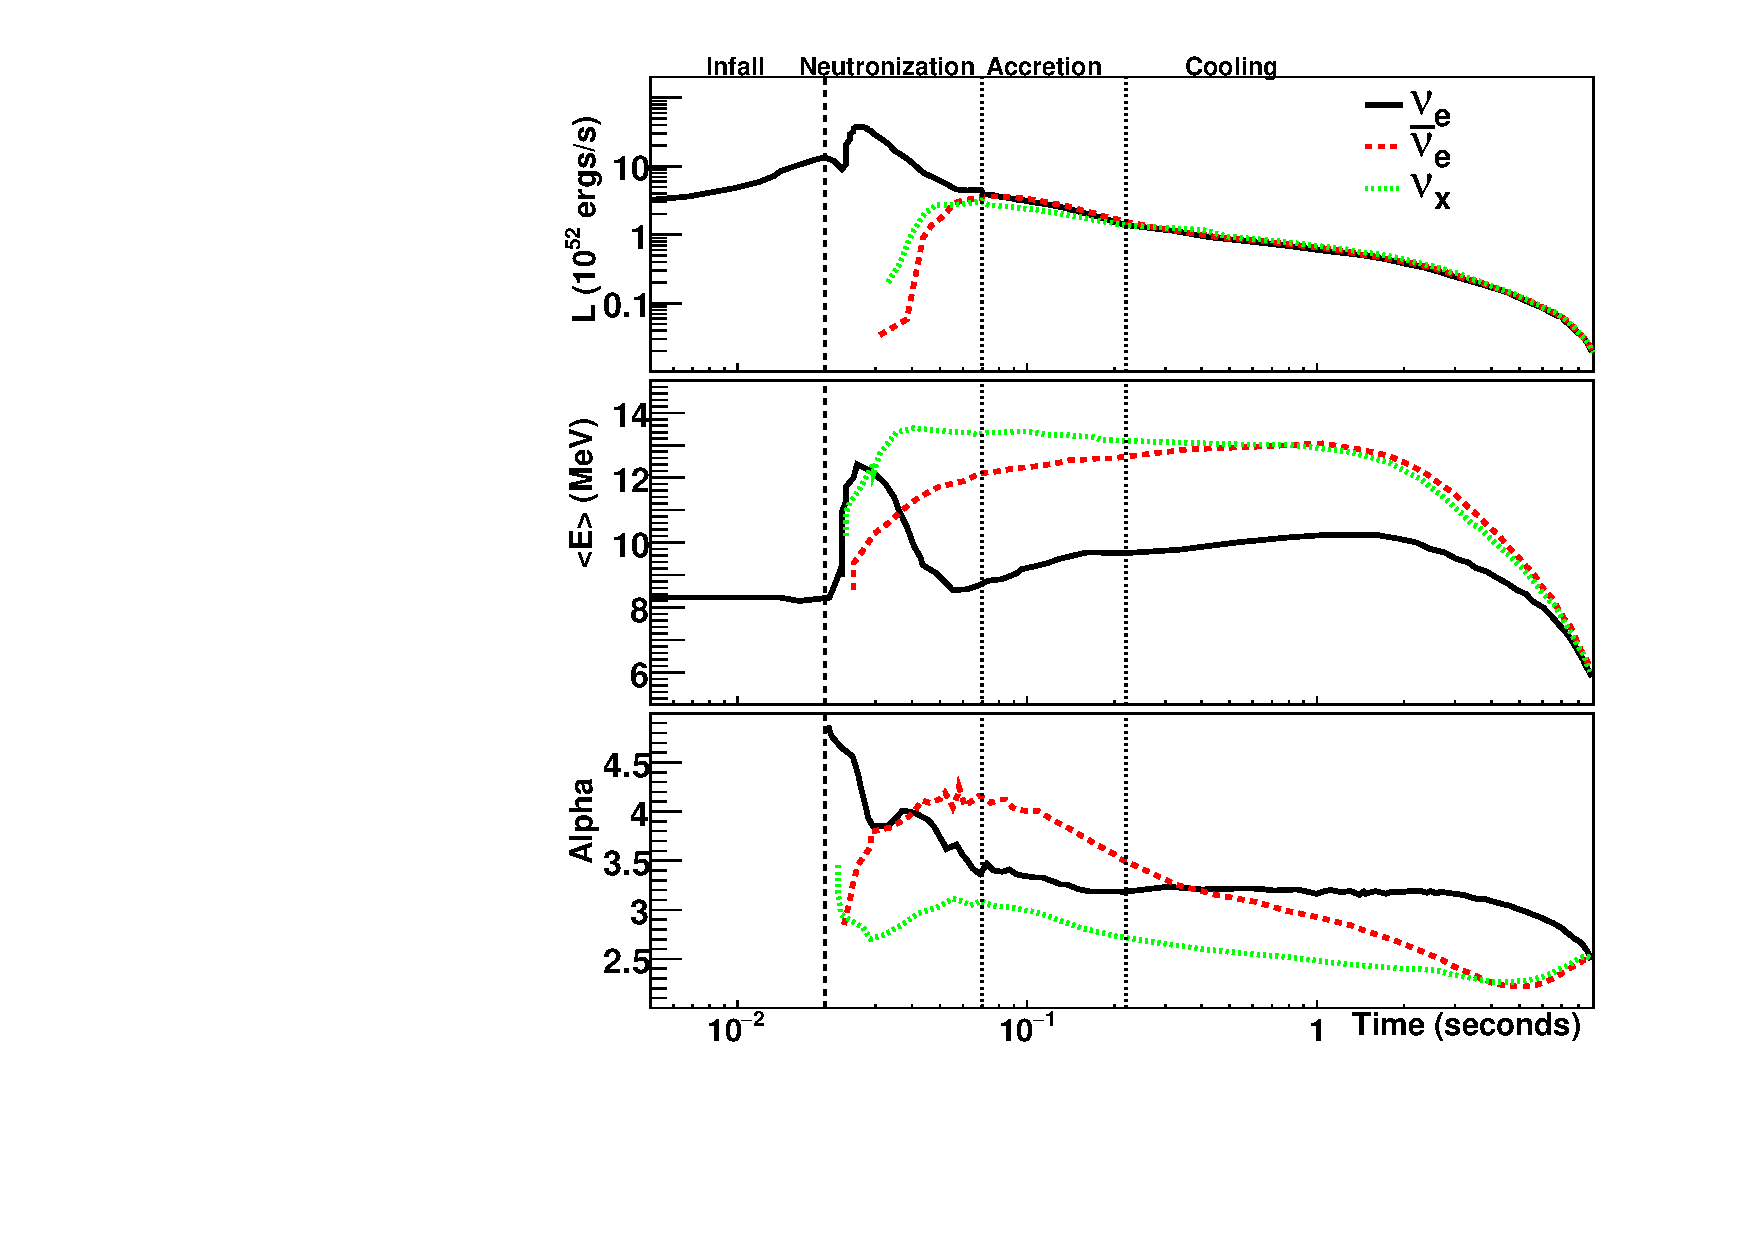
\includegraphics[width=0.9\textwidth]{garching_paramonly.pdf}
\end{dunefigure}

\begin{dunefigure}[Expected fluxess]{3timescales}{Example of time-dependent spectra for the electron-capture supernova model~\cite{Huedepohl:2009wh} parameterized in Figure~\ref{params}, on three different timescales.   The z-axis units are neutrinos per cm$^2$ per millisecond per 0.2~MeV.  Top: $\nu_e$.  Center: $\bar{\nu}_e$.  Bottom: $\nu_x$.  Oscillations are not included here; note they can have dramatic effects on the spectra.}
\centerline{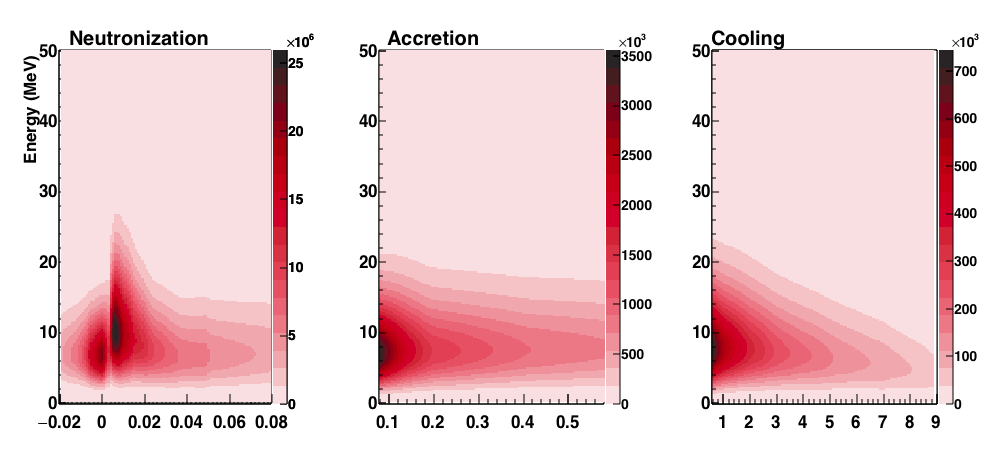
\includegraphics[width=10cm]{garching_nue_flux_3timescales.png}}
\centerline{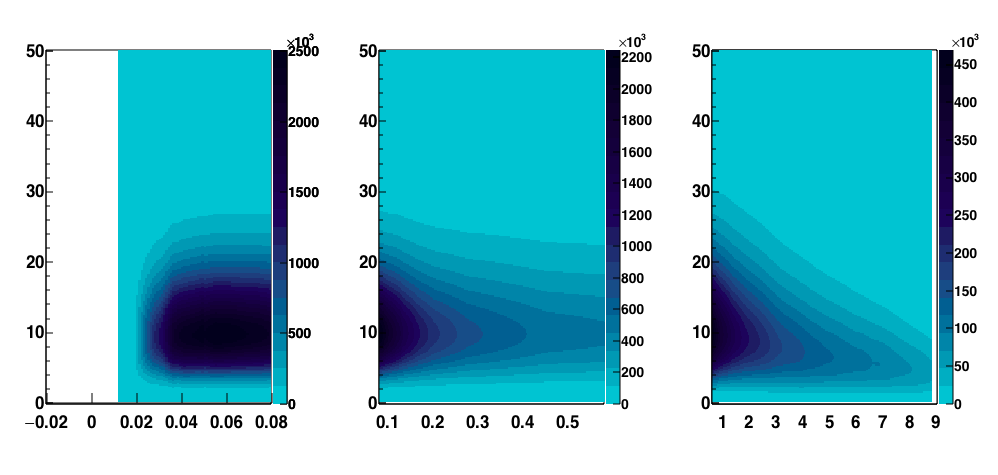
\includegraphics[width=10cm]{garching_nuebar_flux_3timescales.png}}
\centerline{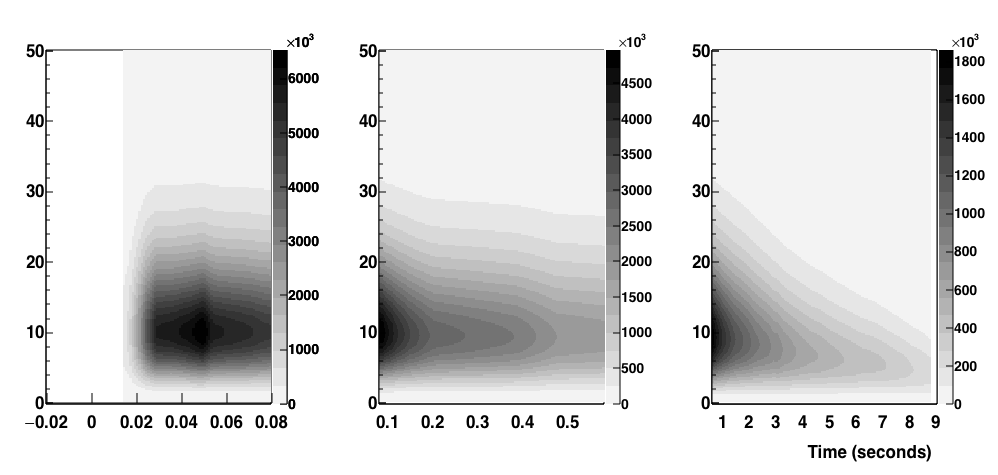
\includegraphics[width=10cm]{garching_nux_flux_3timescales.png}}
\end{dunefigure}

%Figure~\ref{fig:spectrum}, based on a 1-dimensional model of~\cite{Fischer:2009af} and reproduced from~\cite{Wurm:2011zn}.



% \begin{dunefigure}[Expected core-collapse neutrino signal]{spectrum}{Expected
%   core-collapse neutrino signal from the ``Basel''
%   model~\cite{Fischer:2009af}, for a
%   10.8 $M_{\odot}$ progenitor.  The left plots show the very early
%   signal, including ``neutronization burst;'' the middle plots show
%   the ``accretion phase'', and the right plots show the cooling
%   phase. Across the top, luminosities as a function of time are shown. 
%   Across the bottom, the plots show average energy as a function of time for the
%   $\nu_e$, $\overline{\nu}_e$ and $\nu_{\mu,\tau}$ flavor components of the
%   flux (fluxes for $\nu_\mu$, $\overline{\nu}_\mu$, $\nu_\tau$,
%   and $\overline{\nu}_\tau$ should be identical).  Figure courtesy of~\cite{Wurm:2011zn}.}
% 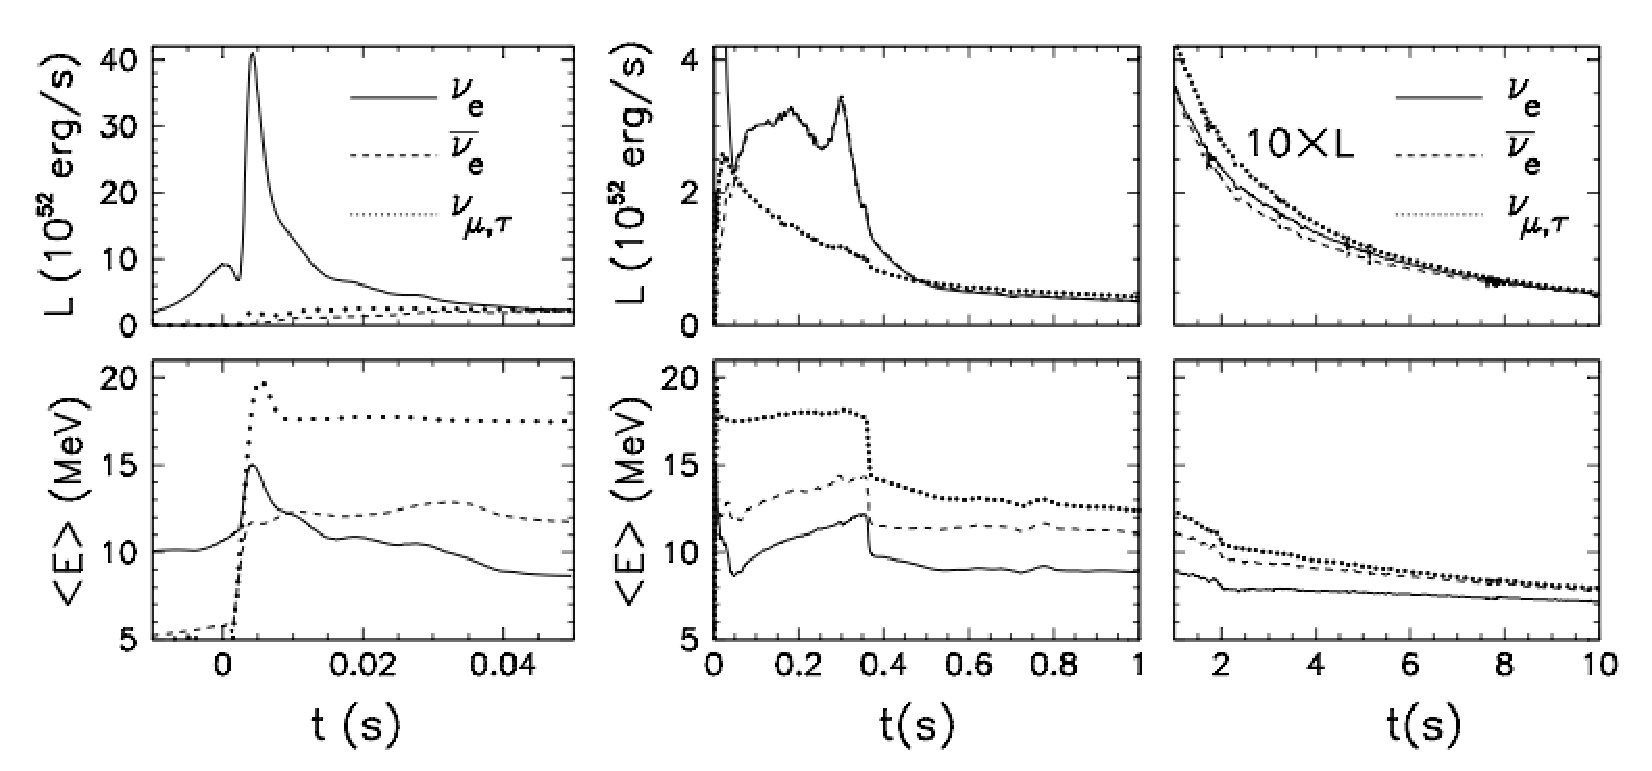
\includegraphics[width=0.9\textwidth]{basel_flux.pdf}
% \end{dunefigure}

The physics of neutrino decoupling and spectra formation is far from trivial, owing to the energy dependence of the cross sections and the roles played by both charged- and neutral-current reactions.
Detailed transport calculations using methods such as \dword{mc} or Boltzmann solvers have been employed. It has been observed that spectra coming out of such simulations can typically be parameterized at a given moment in time by the following ansatz (e.g.,~\cite{Minakata:2008nc,Tamborra:2012ac}):
\begin{equation}
        \label{eq:pinched}
        \phi(E_{\nu}) = \mathcal{N} 
        \left(\frac{E_{\nu}}{\langle E_{\nu} \rangle}\right)^{\alpha} \exp\left[-\left(\alpha + 1\right)\frac{E_{\nu}}{\langle E_{\nu} \rangle}\right] \ ,
\end{equation}
where $E_{\nu}$ is the neutrino energy, $\langle E_\nu \rangle$ is the
mean neutrino energy, $\alpha$ is a ``pinching parameter'', and
$\mathcal{N}$ is a normalization constant.
%
Large $\alpha$ corresponds to a more ``pinched'' spectrum (suppressed
high-energy tail). This parameterization is referred to as a
``pinched-thermal'' form. The different $\nu_e$, $\overline{\nu}_e$ and
$\nu_x, \, x = \mu, \tau$ flavors are expected to have different
average energy and $\alpha$ parameters and to evolve differently in
time. 

The initial spectra get further processed (permuted) by flavor oscillations and understanding these oscillations is very important for extracting physics from the detected signal.


\section{Low-Energy Events in DUNE}\label{sec:lowe-events}

\subsection{Detection Channels and Interaction Rates}

Liquid argon should have a particular sensitivity to the $\nu_e$
component of a supernova neutrino burst, via the dominant interaction,
charged-current
absorption of $\nu_e$ on $^{40}$Ar,
\begin{equation}
\nu_e + ^{40}{\rm Ar} \rightarrow e^- + ^{40}{\rm K^*},
\label{eq:nueabs}
\end{equation}
for which the observable is the $e^-$ plus deexcitation products from the excited $K^*$ final state, as well as a $\bar{\nu}_e$ interaction and elastic scattering on electrons.
Cross sections for the most
relevant interactions are shown in Figure~\ref{xscns}.  It is worth
noting that none of the neutrino-$^{40}$Ar cross sections in this
energy range have been experimentally measured; theoretical
calculations may large uncertainties.

% From Flavio
Another process of interest for supernova detection in \dword{lar} detectors,
not yet fully studied,  is neutral-current  scattering on Ar nuclei by
any type of neutrino: $\nu_x + {\rm Ar} \rightarrow \nu_x + {\rm
  Ar}^*$,  for which the signature is given by the cascade of
deexcitation $\gamma$s from the final state Ar nucleus.  A dominant
9.8-MeV Ar$^*$ decay line has been recently identified as a spin-flip
M1 transition~\cite{Hayes}.   At this energy the probability of
$e^+e^-$ pair production is relatively high, offering a potentially
interesting neutral-current tag.  Other transitions are under investigation.


\begin{dunefigure}[Cross sections for supernova-relevant interactions in argon]{xscns}{Cross sections for supernova-relevant interactions in argon~\cite{GilBotella:2003sz,snowglobes}.}
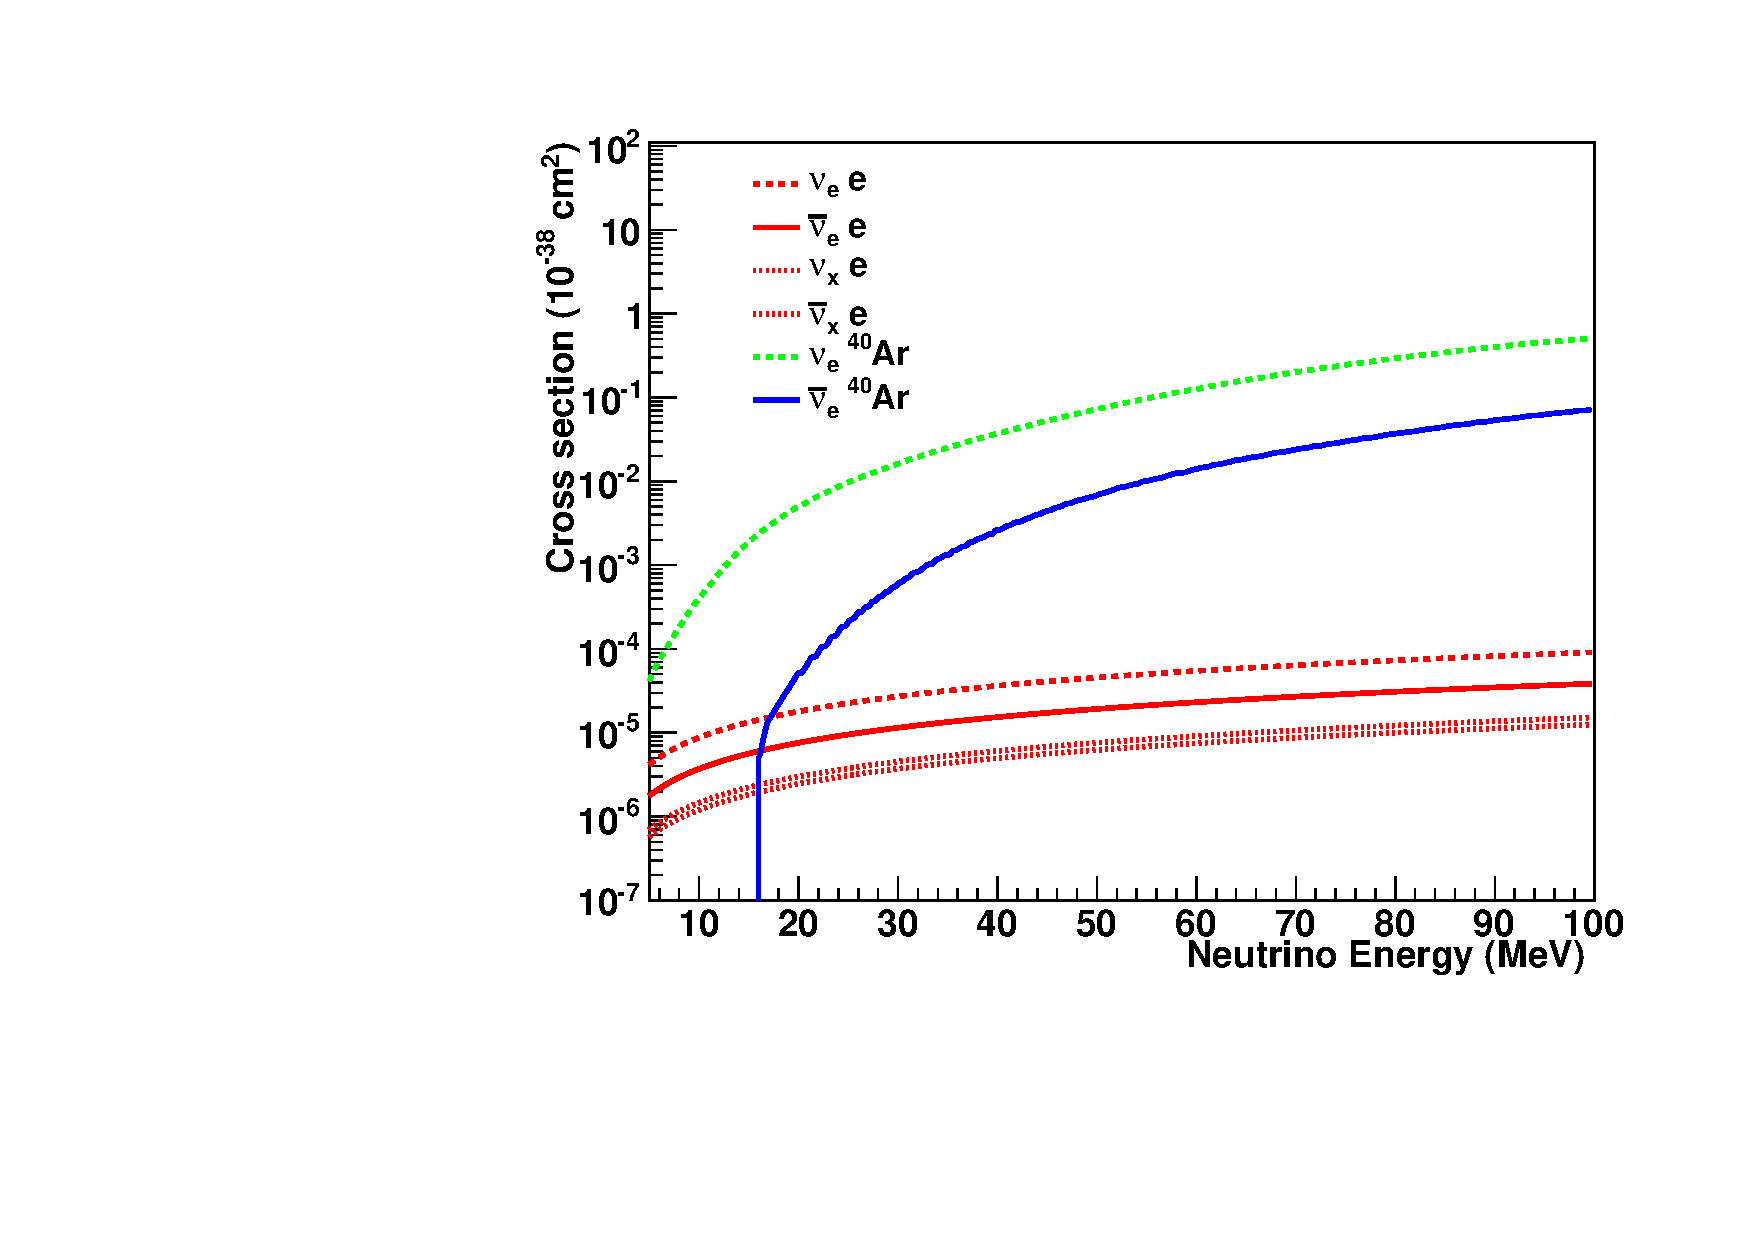
\includegraphics[width=0.6\textwidth]{argon_xscn.pdf}
\end{dunefigure}

The predicted event rate from a supernova burst may be calculated by
folding expected neutrino differential energy spectra with cross
sections for the relevant channels, and with detector response; we do
this using \dword{snowglobes}~\cite{snowglobes} (see Sec.~\ref{snowglobes}.)


\subsection{Event Simulation and Reconstruction}

Supernova neutrino events, due to their low energies, will manifest
themselves primarily as spatially small events, perhaps up to a few tens of cm
scale, with stub-like tracks from
electrons (or positrons from the rarer $\bar{\nu}_e$ interactions).
Events from $\nu_e $ charged-current interactions, $\nu_e+{}^{40}{\rm
  Ar}\rightarrow e^{-}+{}^{40}{\rm K}^{*}$, are likely to be
accompanied by de-excitation products-- gamma rays and/or ejected
nucleons. Gamma-rays are in principle observable via energy deposition
from Compton scattering, which will show up as small charge blips in
the \dword{tpc}.  
Ejected nucleons may result in loss of observed energy for
the event.  Elastic scattering on electrons will result in single
scattered electrons, and single gamma rays may result from \dword{nc} 
excitations of the argon nucleus.   Each event category has, in principle, a
distinctive signature.

The canonical reconstruction task is to identify the interaction
channel, the neutrino flavor for \dword{cc} events, and to determine the
4-momentum of the incoming neutrino; this overall task is the same for
low-energy events as for high-energy ones.  The challenge is to
reconstruct the properties of the lepton (if present), and to the extent
possible, to tag the interaction channel by the pattern of final-state
particles.

% So far, reconstruction algorithms for low-energy neutrinos in DUNE are
% relatively poorly developed with respect to those for high-energy
% events.
While
some physics studies in the \dword{snble} group
 use a fast event-rate calculation tool called \dword{snowglobes}, most
 activity is towards development of realistic and comprehensive
 simulation and reconstruction tools, from neutrino interaction event
 generators through full event reconstruction, in both single and
 dual-phase detectors, with \dword{larsoft}.


\subsubsection{\dshort{marley}}

%MARLEY (Model of Argon Reaction Low Energy Yields)
\dword{marley}~\cite{marley} simulates tens-of-MeV
neutrino-nucleus interactions in liquid argon. Currently, \dword{marley} can only
simulate charged-current $\nu_e$ scattering on $^{40}$Ar, but other
reaction channels will be added in the future.

\dword{marley} weights the incident neutrino spectrum, selects an initial excited state
of the residual $^{40}$K$^*$ nucleus, and samples an outgoing electron
direction using the allowed approximation for the $\nu_e$ \dword{cc} differential cross
section.\footnote{That is, the zero momentum transfer and zero nucleon velocity
limit of the tree-level $\nu_e$ \dword{cc} differential cross section, which may be
written as
\[
\frac{d\sigma}{d\cos \theta}
= \frac{G_F^2 |V_{ud}|^2}{2\pi} |\mathbf{p}_e|\, E_e \,F(Z_f, \beta_e)
\left[(1+\beta_e \cos\theta)B(F) + \left(\frac{3 - \beta_e \cos\theta}
{3}\right)B(GT)\right].
\]
In this expression, $\theta$ is the angle between the incident neutrino and the
outgoing electron, $G_F$ is the Fermi constant, $V_{ud}$ is the quark mixing
matrix element, $F(Z_f, \beta_e)$ is the Fermi function, and $|\mathbf{p}_e|$,
$E_e$, and $\beta_e$ are the outgoing electron's three momentum, total energy,
and velocity, respectively. $B(F)$ and $B(GT)$ are the Fermi and Gamow-Teller
matrix elements.
}
\dword{marley} computes this cross section using a table of Fermi and Gamow-Teller
nuclear matrix elements. Their values are taken from experimental measurements
at low excitation energies and a quasiparticle random phase approximation
(QRPA) calculation at high excitation energies. As the code develops, a more
sophisticated treatment of this cross section will likely be included.

After simulating the initial two-body $^{40}${Ar}($\nu_e$,
$e^{-}$)$^{40}$K$^*$ reaction for an event, \dword{marley}
also handles the subsequent nuclear de-excitation. For bound nuclear
states, the de-excitation $\gamma$-rays are sampled using tables of
experimental branching ratios. These tables are supplemented with
theoretical estimates when experimental data are unavailable. For
particle-unbound nuclear states, \dword{marley} simulates the competition between
$\gamma$-ray and nuclear fragment\footnote{ Nucleons and light nuclei up to
$^{4}${He} are considered.} emission using the Hauser-Feshbach
statistical model.   Figure~\ref{fig:marleydist} shows an example
visualization of a simulated \dword{marley} event.

Although many refinements remain to be made, \dword{marley}'s treatment of high-lying
Gamow-Teller strength and nuclear de-excitations represents a significant
improvement over existing tools for simulating supernova $\nu_e$ \dword{cc} events.  \dword{marley} has been now been fully incorporated into the \dword{larsoft} code base 
and is being used in studies.

%Users who wish to
%perform supernova studies using MARLEY or obtain a copy of MARLEY as a
%standalone tool are encouraged to contact Steven Gardiner
%(\href{mailto:sjgardiner@ucdavis.edu}{sjgardiner@ucdavis.edu}) for more
%information and support.


\begin{dunefigure}[\dword{marley} event]{fig:marleydist}{Visualization of an
    example \dword{marley}-simulated $\nu_e$\dword{cc} event, showing the tracks and energy
    deposition points of the interaction products. }
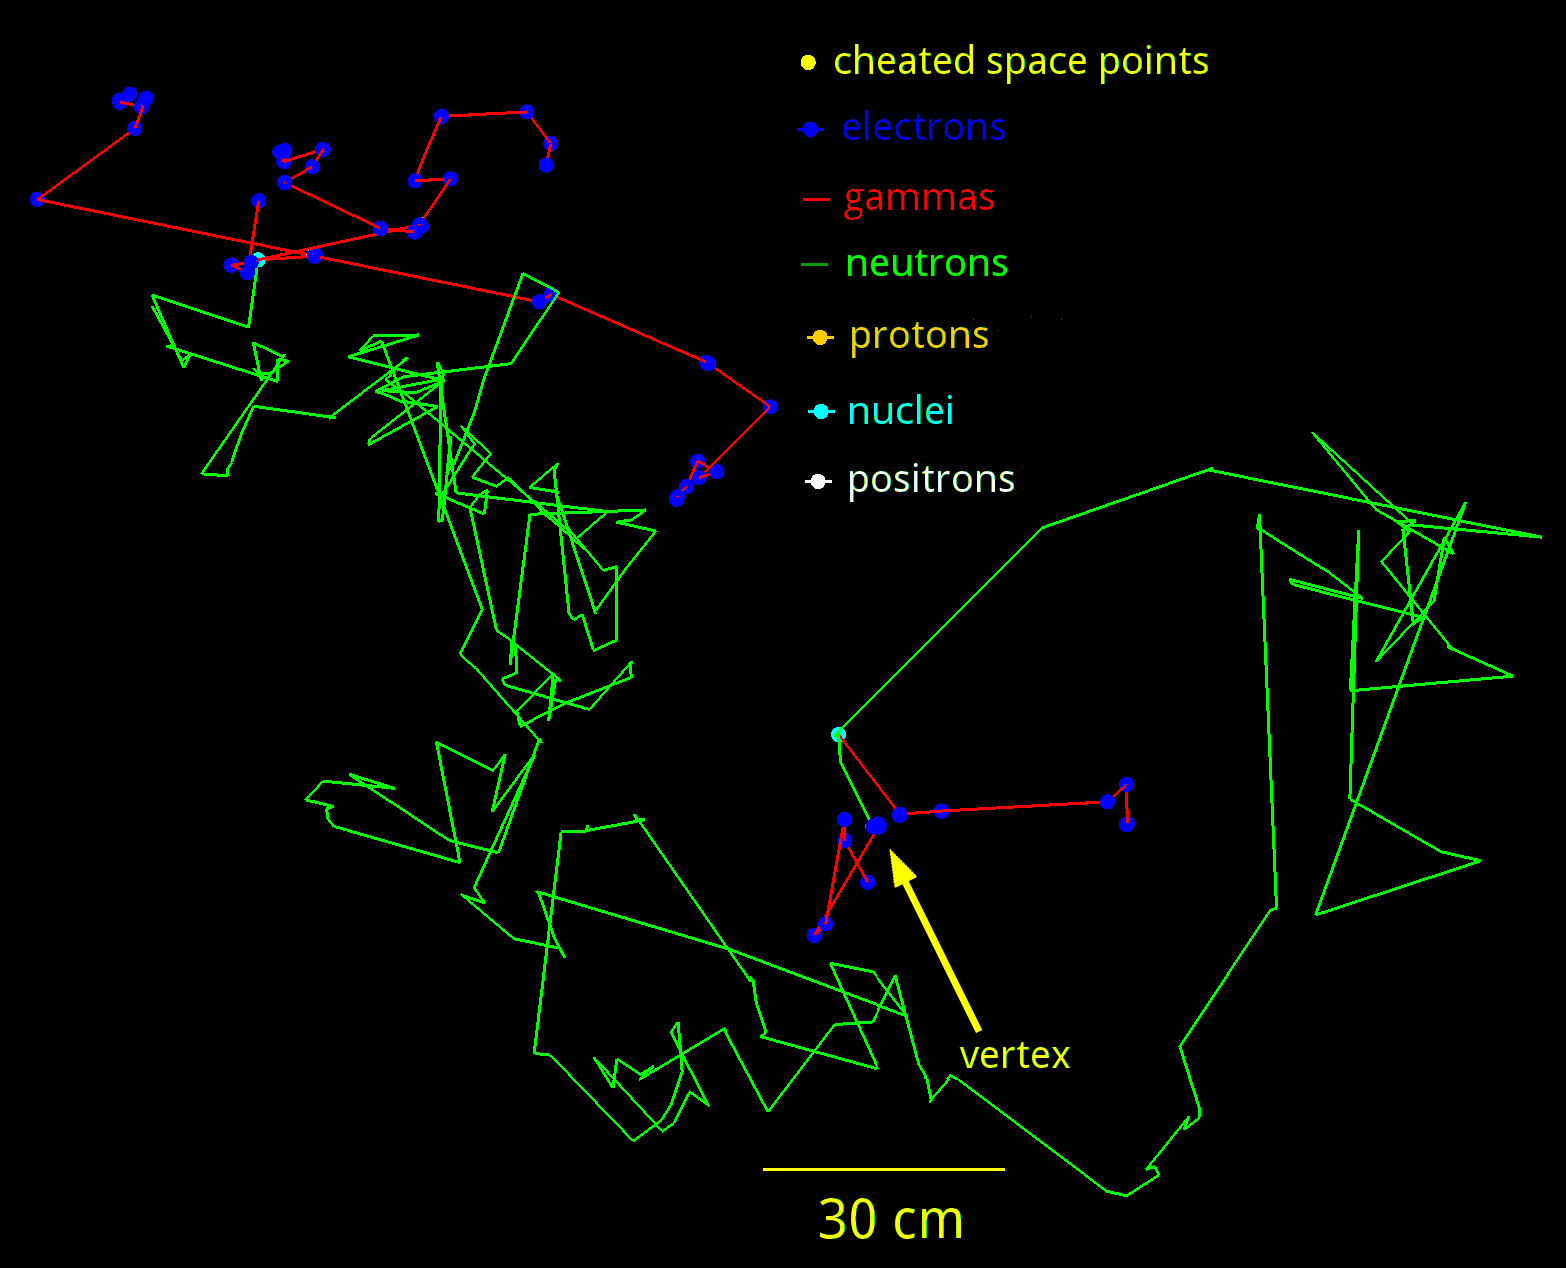
\includegraphics[width=0.6\textwidth]{n_event_tracks-1.png}
\end{dunefigure}


\subsubsection{Low-energy Event Reconstruction Performance}

The standard DUNE reconstruction tools in \dword{larsoft} provide
energy and track reconstruction for
low energy events.  Photons may also be used for calorimetry (see
Sec.~\ref{fixme}).
Figure~\ref{reseff} shows summarized resolution and efficiency for
\dword{marley} events.

\begin{dunefigure}[Resolution and efficiency]{reseff}{Left:
    reconstruction efficiency as a function of neutrino energy for
    MARLEY events, for different minimum required reconstructed
    energy. Right: fractional energy resolution as a function of
    neutrino energy for TPC tracks (black) and photon detector
    calorimetry (blue). The red ``physics-limited resolution'' assumes
  all energy deposited by final-state particles is reconstructed; the
  finite resolution represents loss of energy from escaping particles.}
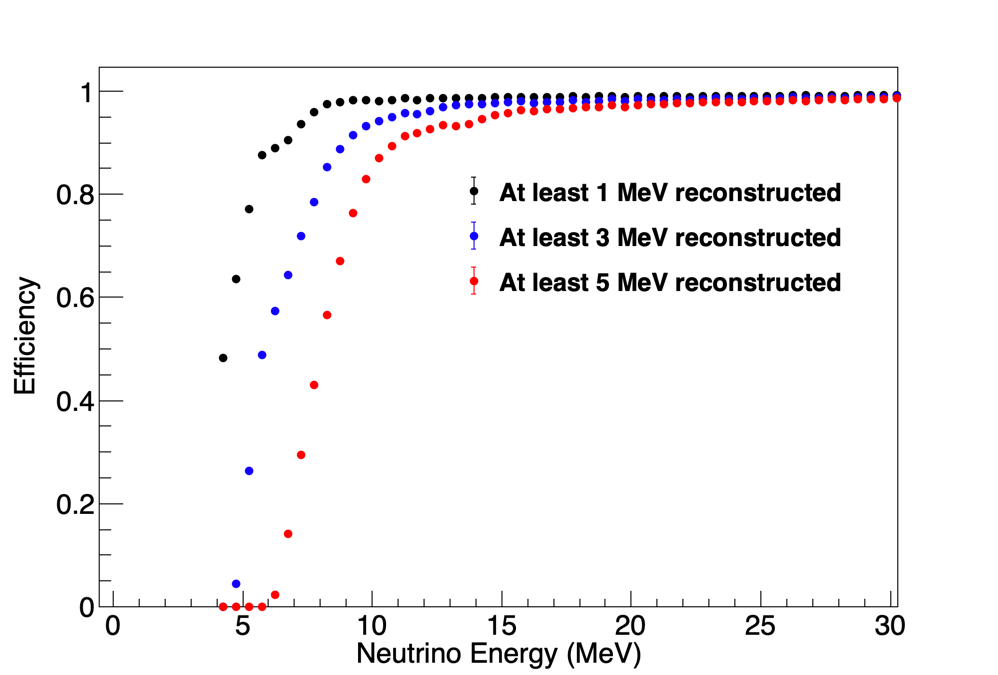
\includegraphics[width=0.45\textwidth]{EfficVsNeutrinoEnergy.png}
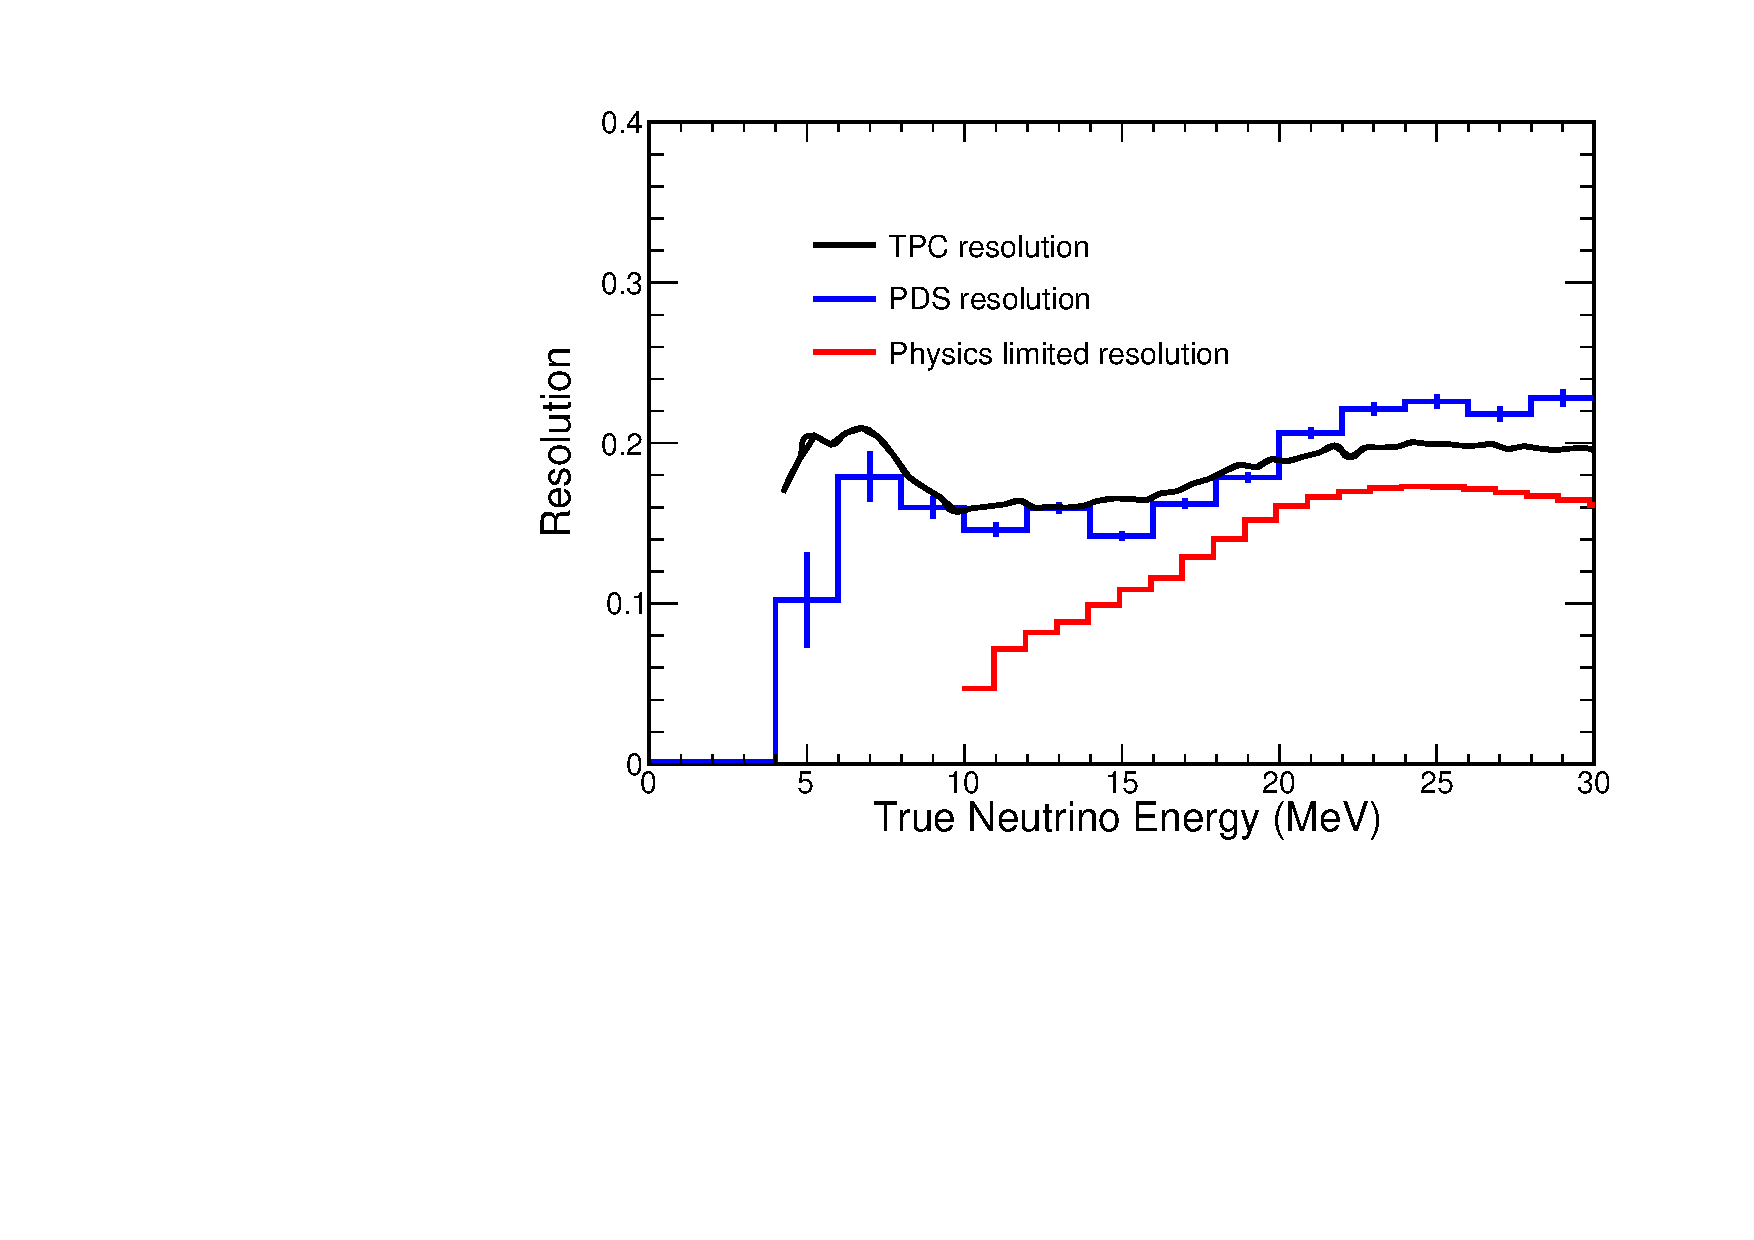
\includegraphics[width=0.45\textwidth]{pds-snb-res-vs-truex_optimized.pdf}
\end{dunefigure}



\subsubsection{ \dword{snowglobes}}\label{snowglobes}

Most supernova neutrino studies done for DUNE so far, including of the
plots included in the \dword{cdr}~\cite{Acciarri:2015uup}, have employed
 \dword{snowglobes}\cite{snowglobes}, a fast event-rate computation tool.  This
uses %$\globes$
\dword{globes} front-end software~\cite{Huber:2004ka,globes} to
convolve fluxes with cross-sections and detector parameters.  The
output is in the form of interaction rates for each channel as a
function of neutrino energy, and ``smeared'' rates as a function of
detected energy for each channel (i.e., the spectrum that
actually be observed in a detector).  
The smearing (transfer) matrices incorporate both
interaction product spectra for a given neutrino energy, and detector
response.   Figure~\ref{marleysmearing} shows such a transfer matrix
created
using \dword{marley}, by determining the distribution of observed charge, and
 a full simulation of the detector response (including the generation,
 transport, and detection of ionization signals and the electronics)
 as a function of neutrino energy in 0.5-MeV neutrino energy steps.
Time dependence in  \dword{snowglobes} can be straightforwardly
handled by providing multiple files with fluxes divided into different
time bins. \footnote{Note that  \dword{snowglobes} is \textit{not} a \dlong{mc}
code--- it calculates mean event rates using a transfer matrix to
convert neutrino spectra to observed spectra.  This will produce
equivalent results to reweighting Monte Carlo.}


% For default SNOwGLoBES, a
% detection threshold of 5 MeV in LAr is assumed as well as energy resolution
% from Ref.~\cite{Amoruso:2003sw}.    Furthermore, the current default detector
% response smearing for LAr in SNOwGLoBES  assumes that all energy from
% de-excitation products is captured, which is likely a poor assumption. 
% User-created transfer matrices have also been used
% for some studies~\cite{gleb, glebdocdb}.


\begin{dunefigure}[\dword{marley} event]{marleysmearing}{Smearing matrix for
     \dword{snowglobes} created with monochromatic \dword{marley} samples run though
    \dword{larsoft}, describing detected charge distribution as a function of
    neutrino energy.  The effects of interaction product distributions
  and detector smearing are both incorporated in this matrix.  The
  right hand plot 
  incorporates an assumed drift correction based on \dlong{mc} truth.}
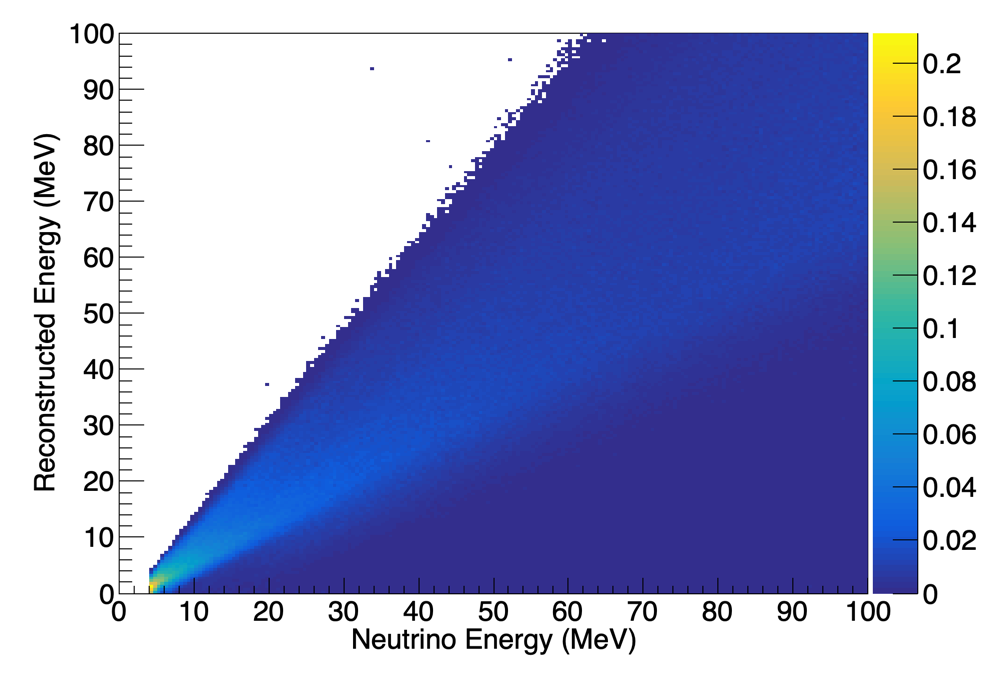
\includegraphics[width=0.45\textwidth]{smear_nue_Ar40_ar40kt_NoDC_Centered.png}
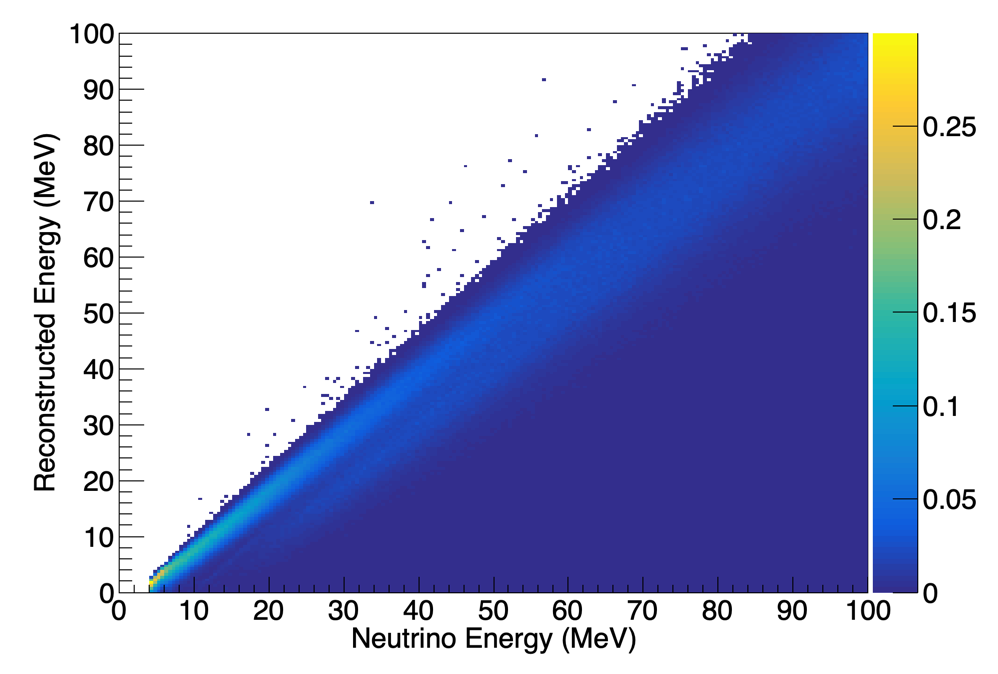
\includegraphics[width=0.45\textwidth]{smear_nue_Ar40_ar40kt_DCT_Centered.png}

% 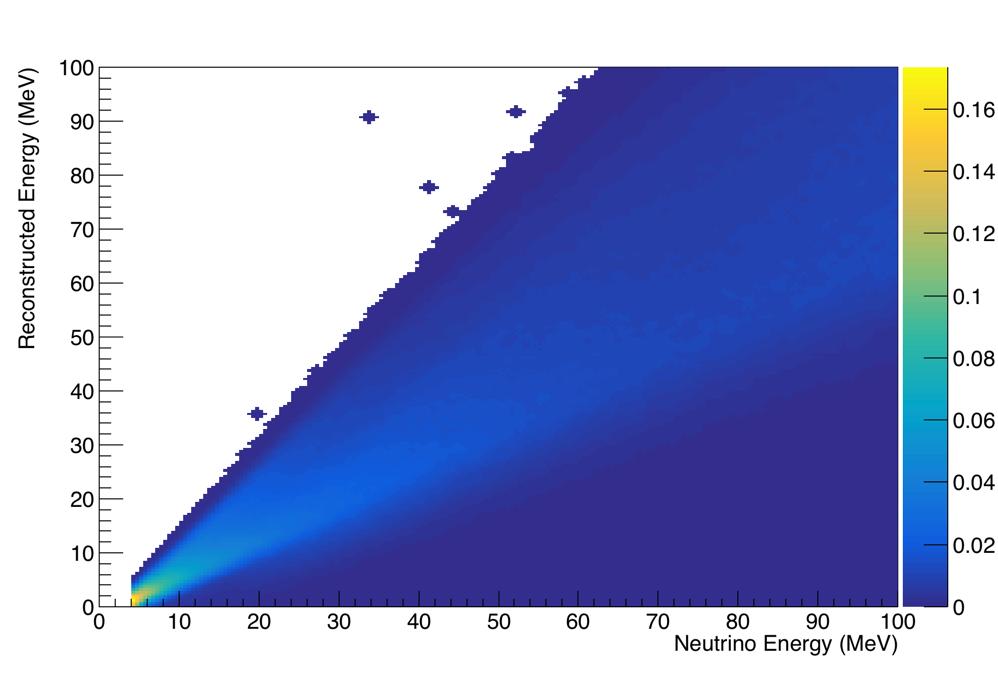
\includegraphics[width=0.4\textwidth]{SmearingMatrix_HitIntegral_TDR.png}
%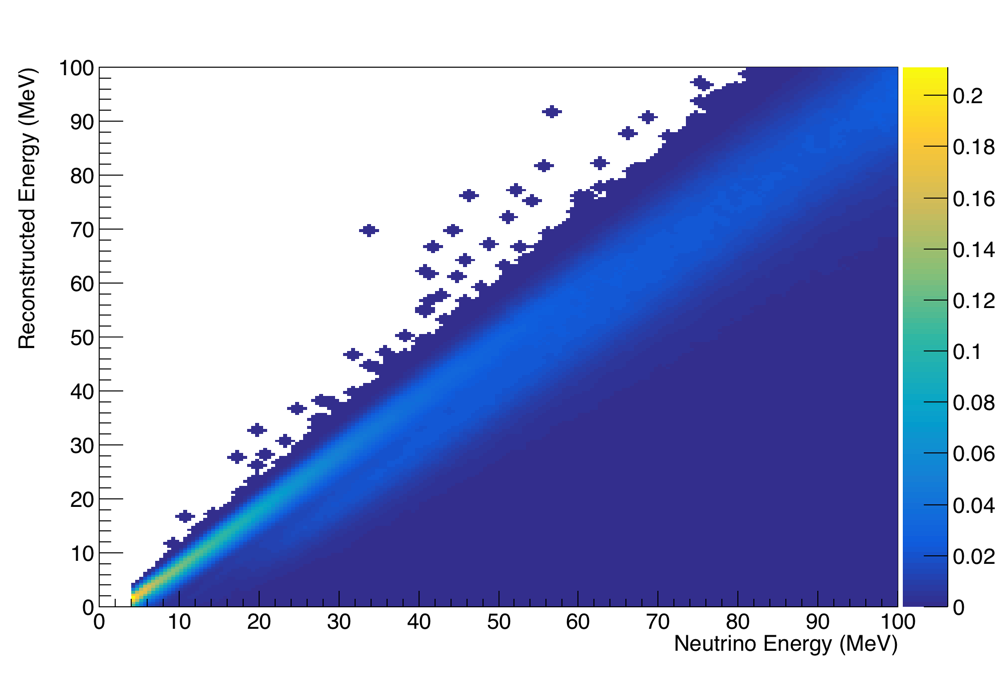
\includegraphics[width=0.4\textwidth]{SmearingMatrix_HitIntegral_DCT_TDR.png}
\end{dunefigure}


While \dword{snowglobes} is, and will continue to be, a fast, useful tool,
it has limitations with respect to a full simulation.  One loses correlated
event-by-event angular and energy information, for example; some
studies, such as the directionality study in
Section~\ref{sec:pointing} require such complete event-by-event information.
Nevertheless, transfer matrices generated with the best available
simulations can be used to compute observed event rates and energy distributions and draw useful conclusions.
%Ideally one does studies with high-statistics simulated data with
%realistic event generators and detector response.
%When full simulation studies are constrained by computational resources,
%one can update transfer matrices using improved simulation and still use
%SNOwGLoBES to draw useful conclusions.


\subsubsection{Backgrounds}

Understanding of backgrounds is also critical for understanding of how
well we can reconstruct low energy events, and for setting detector
requirements.  Small single-hit blips from $^{39}$Ar or other
impurities may fake de-excitation gammas.  While preliminary studies
show that backgrounds will have a minor effect on reconstruction of
triggered supernova burst events, their effects on a \dword{daq} and
triggering system that satisfies supernova burst triggering
requirements is significant.  Furthermore backgrounds matter for
selection of low-rate events such as solar neutrinos.
Sections~\ref{bg, DAQ} discuss these issues further.

% Backgrounds may be especially important for photon
% detectors (which in turn may be important for energy resolution by
% correcting for attenuation of charge during drift)--- see
% Section~\ref{sec:snb_photons}.
% Work on
% backgrounds is done in collaboration with the DUNE Radiopurity group.

\section{Expected Supernova Burst Signal Properties}\label{sec:sn-signals}


Table~\ref{argon_events} shows rates calculated  for the dominant interactions in argon for
the ``Livermore'' model~\cite{Totani:1997vj} (out of date, but included for comparison with literature), and the ``GKVM''
model~\cite{Gava:2009pj}; for the former, no oscillations are assumed; the latter assumes collective effects.  In general, there is a rather wide variation--- up to an order of magnitude --- in event rate for different models, due to different numerical treatment (e.g., neutrino transport, dimensionality), physics input (nuclear equation of state, nuclear correlation and impact on neutrino opacities, neutrino-nucleus interactions) and oscillation effects. In addition, there is intrinsic variation in the nature of the progenitor and collapse mechanism.  Neutrino emission from the supernova may furthermore have an emitted lepton-flavor asymmetry~\cite{Tamborra:2014aua}, so that observed rates may be dependent on the supernova direction.
\begin{dunetable}[Event numbers for different models in \SI{40}{\kt} of \dword{lar} for
    a core-collapse at 10~kpc]{lcc}{argon_events}{Event counts for different
    supernova models in \SI{40}{\kt} of liquid argon for a core collapse at 10~kpc, for $\nu_e$ and $\bar{\nu}_e$ charged-current channels and \dword{es} on electrons.
    Event rates will simply scale by active detector mass and inverse
    square of supernova distance.   No oscillations are assumed; we
    note that oscillations (both standard and ``collective'') will
    potentially have a large, model-dependent effect, discussed in Sec.~\ref{sec:mh}.}
Channel & Events & Events \\
\rowtitlestyle
& ``Livermore'' model & ``GKVM'' model  \\ 
\toprowrule

$\nu_e + ^{40}{\rm Ar} \rightarrow e^- + ^{40}{\rm K^*}$ & 2720  & 3350 \\ \colhline

$\overline{\nu}_e + ^{40}{\rm Ar} \rightarrow e^+ + ^{40}{\rm Cl^*}$ & 230 & 160\\ \colhline

$\nu_x + e^- \rightarrow \nu_x + e^-$                           & 350 &  260\\ \colhline

Total &  3300 & 3770 \\ 
\end{dunetable}



% Figure~\ref{fig:garching} gives another example of an expected burst
% signal, for which a calculation with detailed time dependence of the
% spectra is available~\cite{Huedepohl:2009wh} out to 9~seconds
% post-bounce.  This model has relatively low luminosity but the standard robust
% neutronization burst.  Note that the relative fraction of
% neutronization-burst events is quite high.
% Figure~\ref{fig:eventrates} shows the event channel breakdown for the
% same model.

Clearly, the $\nu_e$
flavor dominates.  Although water and scintillator detectors will record $\nu_e$ events~\cite{Laha:2013hva,Laha:2014yua}, liquid argon is the only future prospect for a large, clean supernova $\nu_e$ sample~\cite{Scholberg:2012id}.


% \begin{dunefigure}[Garching flux signal with neutronization burst]{garching}{Expected
%   time-dependent signal for a specific flux model for an
%   electron-capture supernova~\cite{Huedepohl:2009wh} at 10~kpc.  No oscillations are assumed. The
%   top plot shows the luminosity as a function of time, the second plot
%   shows average neutrino energy, and the third plot shows the $\alpha$
%   (pinching) parameter.  The fourth (bottom) plot shows the total number of
%   events (mostly $\nu_e$) expected in 40 kt of liquid argon, calculated using
%   SNOwGLoBES.  Note the logarithmic binning in time; the plot shows
%   the number of events expected in the given bin and the error bars
%   are statistical. The vertical dashed line at 0.02 seconds indicates
%   the time of core bounce, and the vertical lines indicate different
%   eras in the supernova evolution.  The leftmost time interval
%   indicates the infall period.  The next interval, from core bounce to
%   50~ms, is the neutronization burst era, in which the flux is
%   composed primarily of $\nu_e$.  The next period, from 50 to 200~ms,
%   is the accretion period. The final era, from 0.2 to 9~seconds, is
%   the proto-neutron-star cooling period.}
% 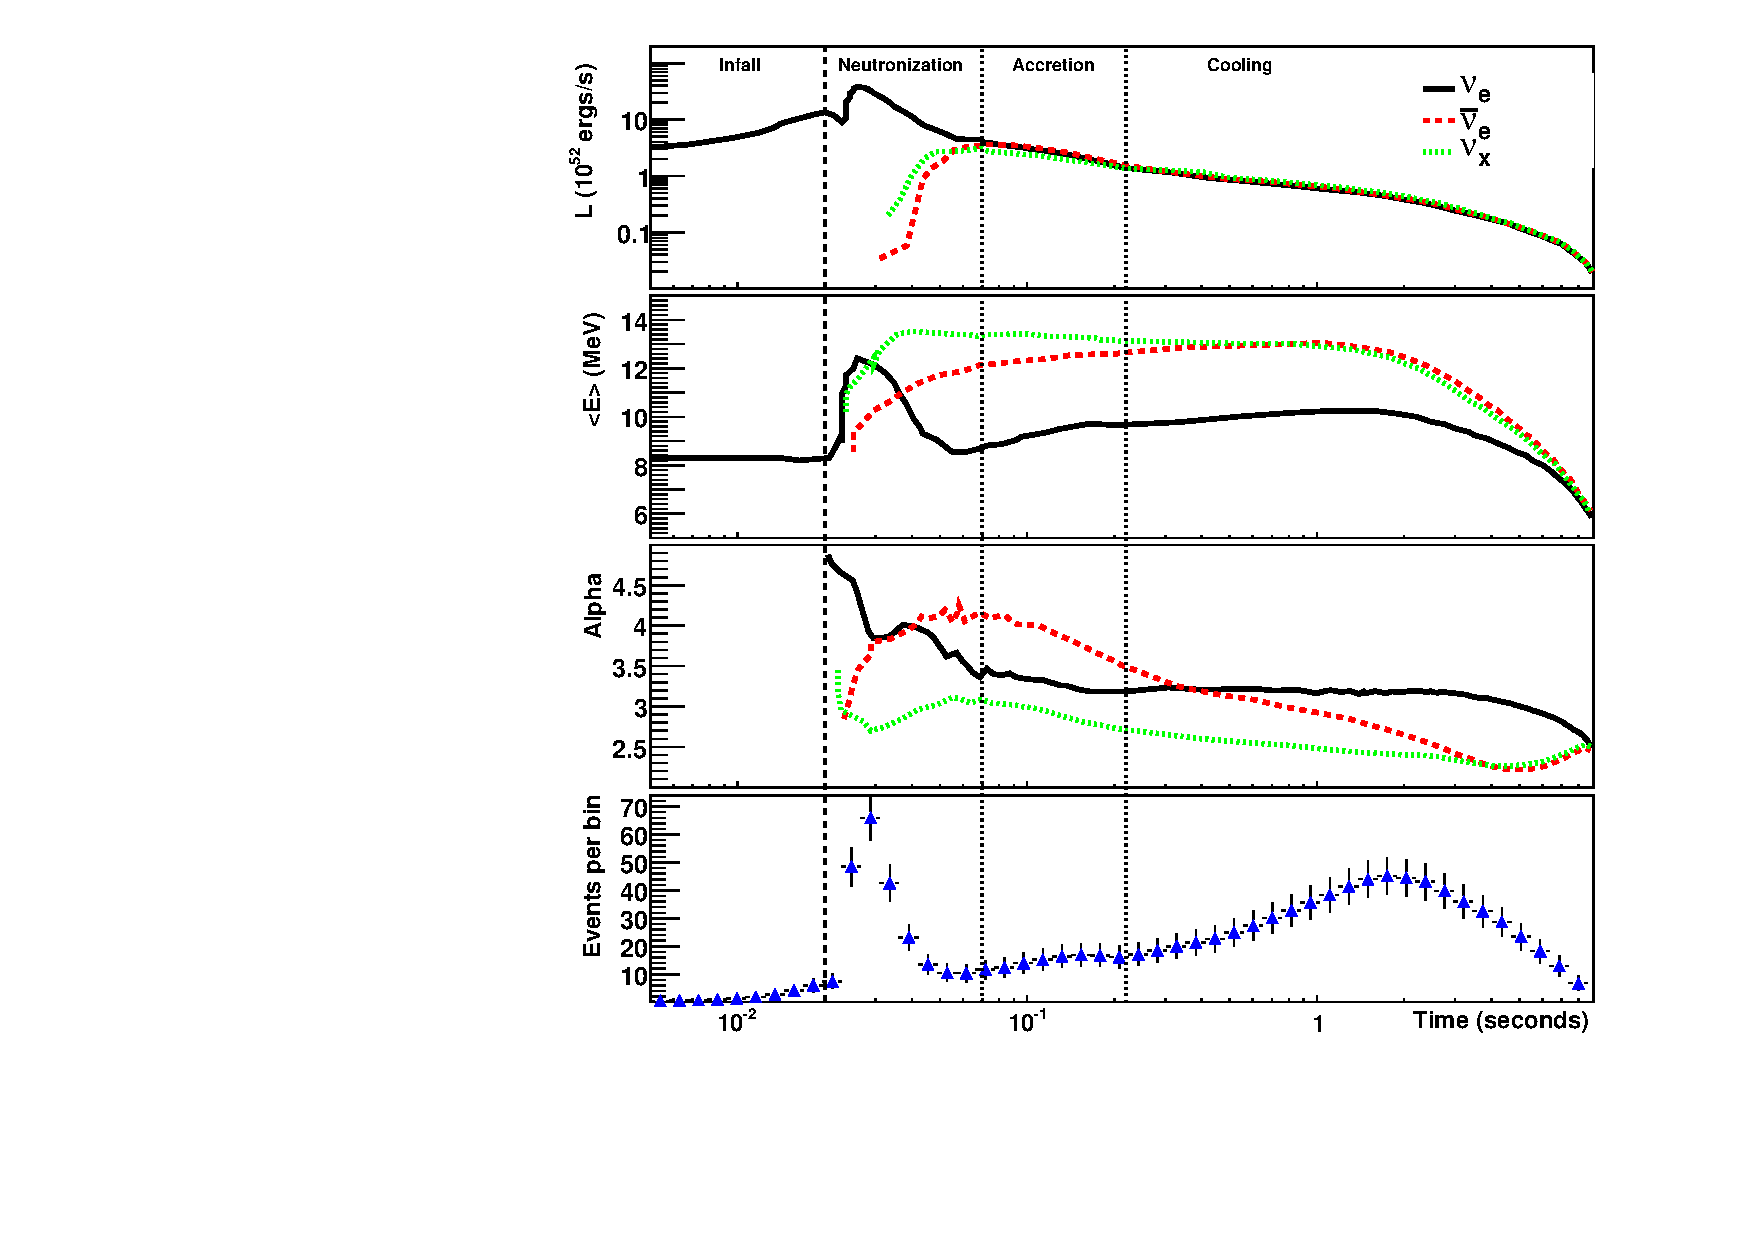
\includegraphics[width=0.9\textwidth]{garching.pdf}
% \end{dunefigure}


% \begin{dunefigure}[Supernova $\nu$ event rates in \SI{40}{kt} of LAr for Garching flux]{eventrates}{Left: Expected
%   time-dependent signal in 40 kt of liquid argon for the electron-capture supernova~\cite{Huedepohl:2009wh} at 10~kpc, calculated using SNoWGLoBES~\cite{snowglobes}, showing breakdown of event channels.  Right: expected measured event spectrum for the same model, integrated over time.}
% %\includegraphics[width=2.5in]{garching_time_plot.pdf}
% %\includegraphics[width=2.5in]{garching_energy_plot.pdf}
% \end{dunefigure}

The number of signal events scales with mass and inverse square of distance as shown in Figure~\ref{ratesvsdist}.  For a collapse in the Andromeda galaxy, a 40-kton detector would observe a few events.

\begin{dunefigure}[Supernova neutrino rates vs distance]{ratesvsdist}{Estimated numbers of supernova neutrino interactions in DUNE as a function of distance to the supernova, for different detector masses ($\nu_e$ events dominate). The red dashed lines represent expected events for a 40-kton detector and the green dotted lines represent expected events for a 10-kton detector. The lines limit a fairly wide range of possibilities for ``Garching-parameterized'' supernova flux spectra (Equation~\ref{eq:pinched}) with luminosity $0.5\times 10^{52}$ ergs over ten seconds. The optimistic upper line of a pair gives the number of events for average $\nu_e$ energy of $\langle E_{\nu_e}\rangle =12$~MeV, and ``pinching'' parameter $\alpha=2$; the pessimistic lower line of a pair gives the number of events for $\langle E_{\nu_e}\rangle=8$~MeV and $\alpha=6$. (Note that the luminosity, average energy and pinching parameters will vary over the time frame of the burst, and these estimates assume a constant spectrum in time. Oscillations will also affect the spectra and event rates.) The solid lines represent the integrated number of events for the specific time-dependent neutrino flux model in~\cite{Huedepohl:2009wh} (see Figures~\ref{params} and \ref{3timescales}; this model has relatively cool spectra and low event rates). Core collapses are expected to occur a few times per century, at a most-likely distance of around 10 to 15 kpc.}
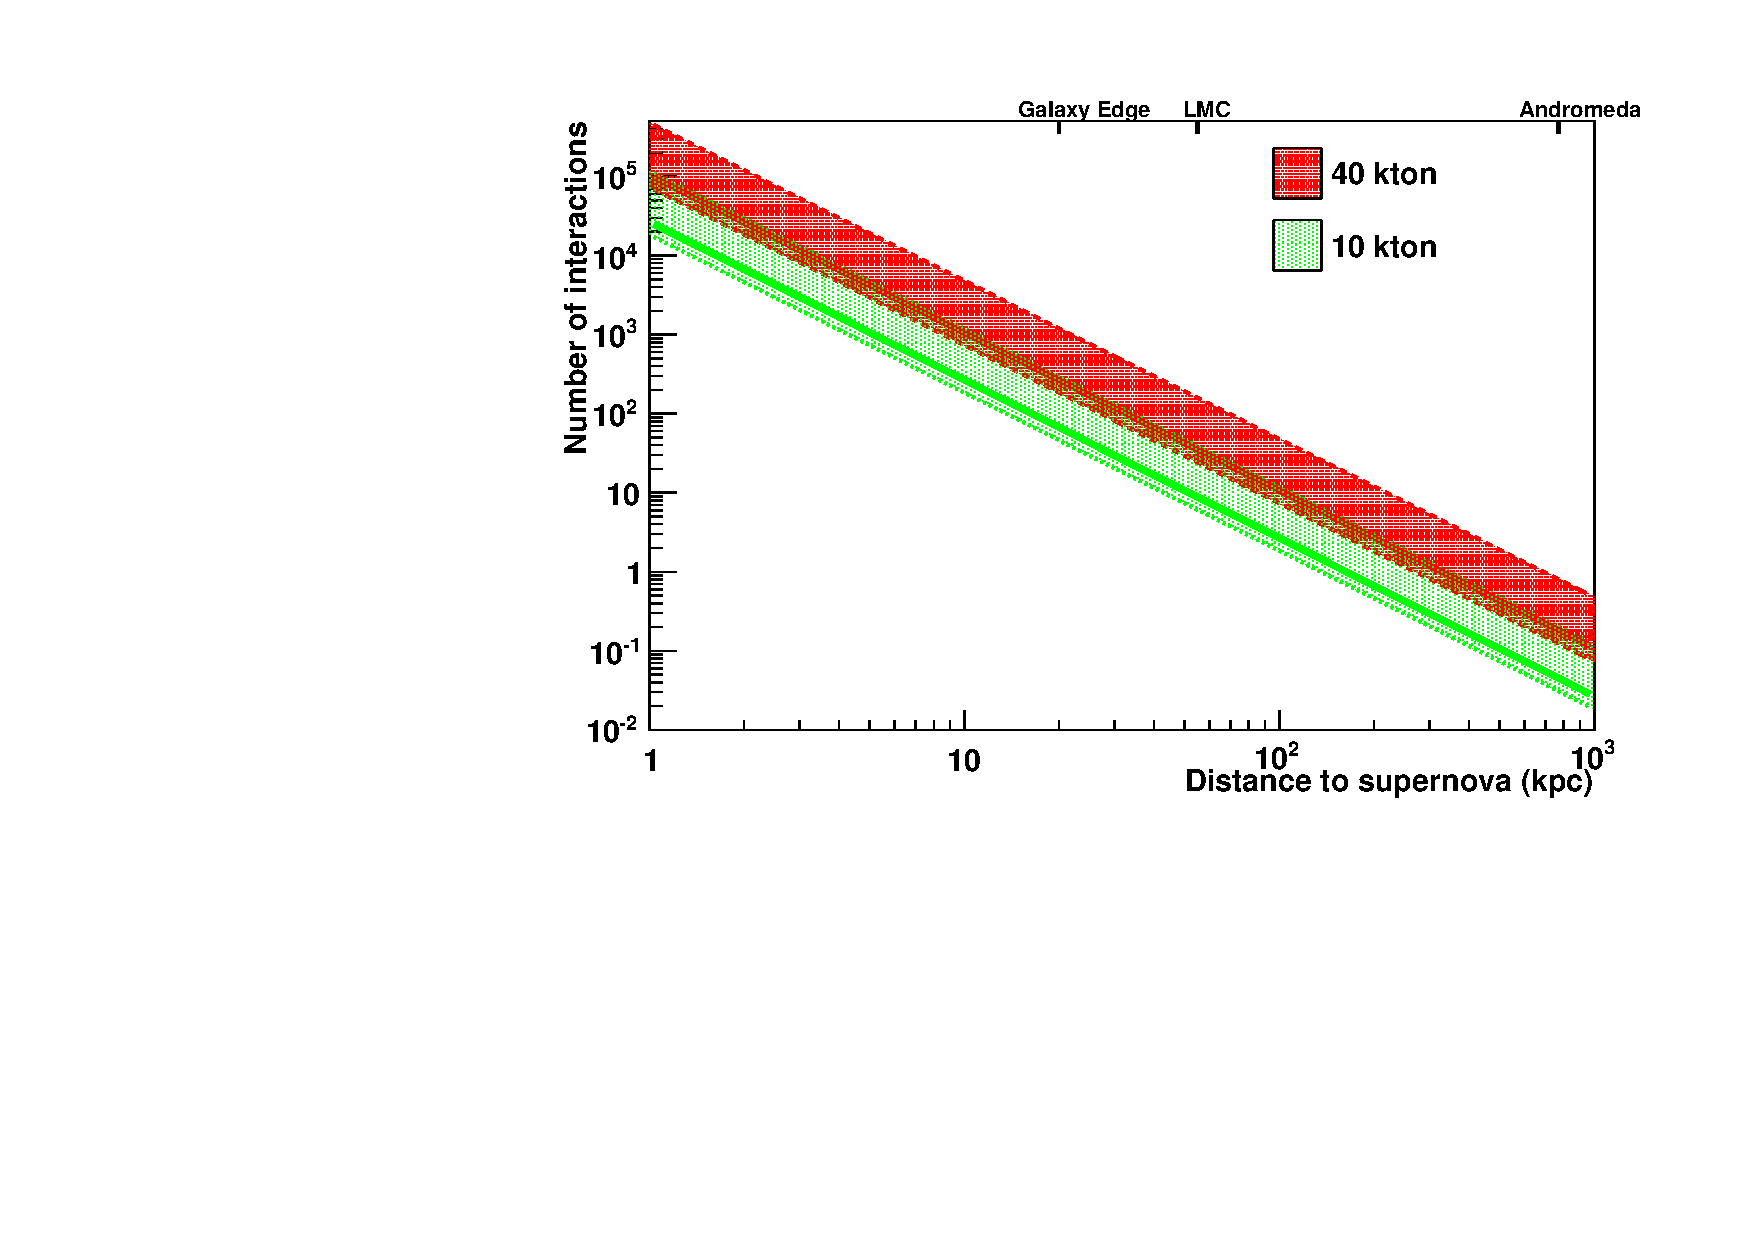
\includegraphics[width=5in]{argon_sn.pdf}
\end{dunefigure}


\subsection{Directionality: pointing to the supernova}\label{sec:pointing}

% Material from AJ Roeth


It will be valuable to use DUNE's tracking ability to reconstruct the direction of the incoming neutrinos to the extent possible.  Reconstruction of direction to a supernova (or other astrophysical event) will be of obvious use to astronomers for prompt detection of the early turn-on of the light.  Furthermore, some core collapse events may not yield bright electromagnetic fireworks, in which case directional information may help in location of a dim even or even a ``disappeared'' progenitor~\cite{Kochanek:2008mp}.
Directional information can be used for correlation with gravitational
wave observations, which also have some directionality.  Pointing
resolution for low-energy events will also be helpful for selecting
signal from background for solar neutrinos or other sources with known
angular distribution.  The directional information could also
potentially be used in a high-level trigger.

The pointing resolution incorporates intrinsic angular spread of the
interaction products of the neutrino interaction, as well as
resolution for detector reconstruction.  A large fraction of the
events expected from the supernova will not point well; in particular,
the expected angular distribution of the $\nu_e$ \dword{cc} absorption
events which will make up the bulk of the signal events are expected
to have relatively weak anisotropy.  In contrast, the elastic
scattering component of the signal should point reasonably well.

We describe here a study of the ability of DUNE to point to a
supernova using the \dword{tpc} tracks.  This study makes use of full 
simulation and reconstruction tools.
We have studied single electrons, neutrino-electron elastic scattering
events, and the full expected supernova signal, looking only at elastic
scattering events.  Future studies will incorporate all interaction
channels, as well as backgrounds.


\begin{dunefigure}[\dword{es} event]{fig:1eevd}{Example event display for a
    single simulated 10.25~MeV electron, with track reconstruction, in
    time vs wire, with color representing charge.
    The top panel shows the collection plane and the bottom panels
    show induction planes.  The boxes represent reconstructed hits. }
 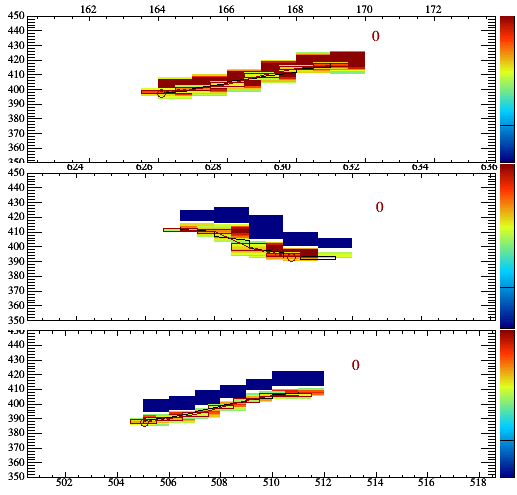
\includegraphics[width=0.4\textwidth]{ES_10-25MeV_Event9001_TDR.png}
\end{dunefigure}


\begin{dunefigure}[Pointing vs neutrino
  energy]{fig:ESpointres}{ Left: Pointing resolution for electron
    tracks, showing effect of direction ambiguity, which can be
    partially resolved using bremsstrahlung directionality. Right: Pointing resolution of elastic scattering
    events versus neutrino energy for each neutrino flavor.}
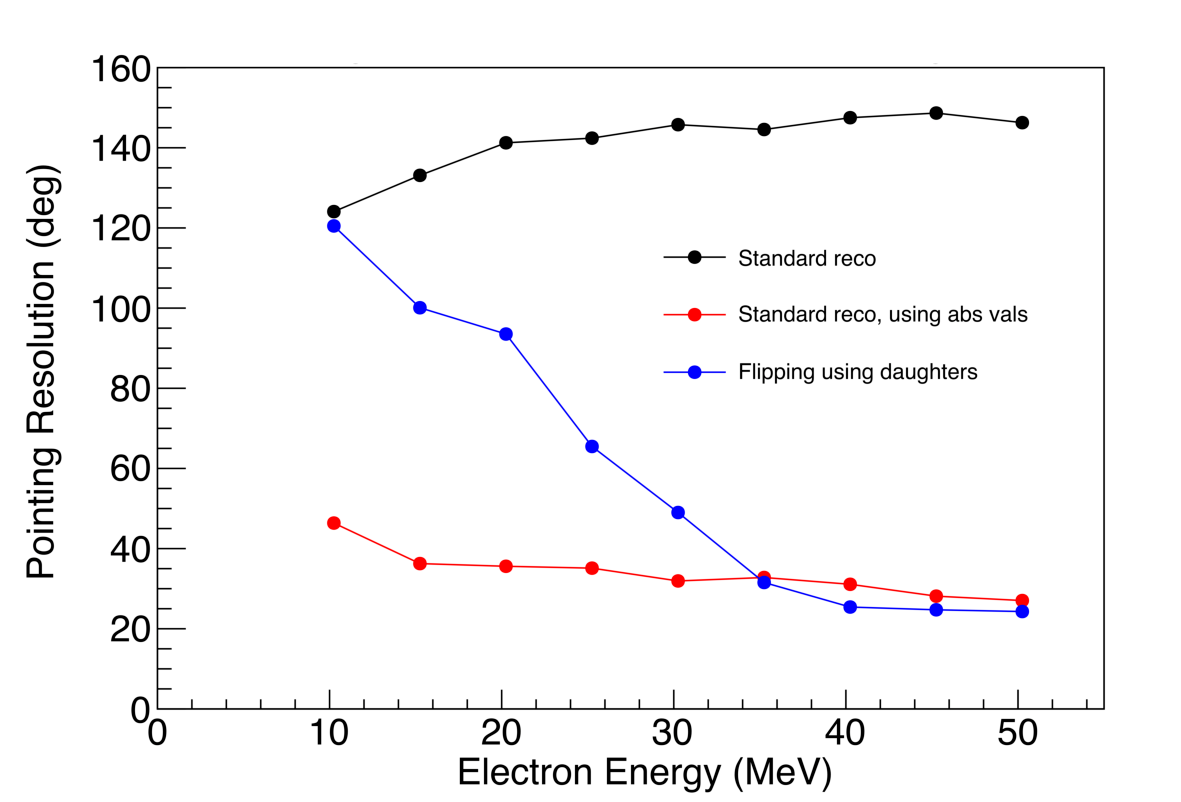
\includegraphics[width=0.4\textwidth]{pointres_vs_energy_1e_dflip2.pdf}
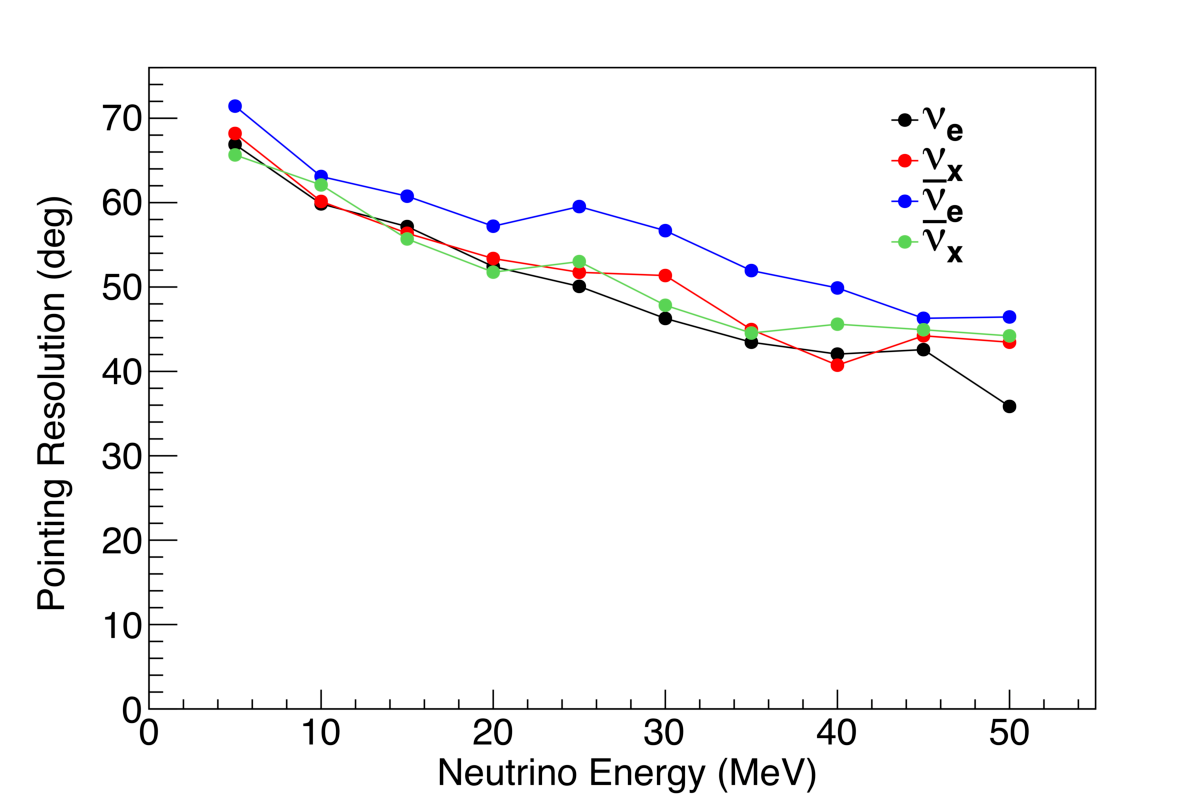
\includegraphics[width=0.4\textwidth]{pointres_vs_energy_ES_reco_abs_PMdQdx.pdf}
%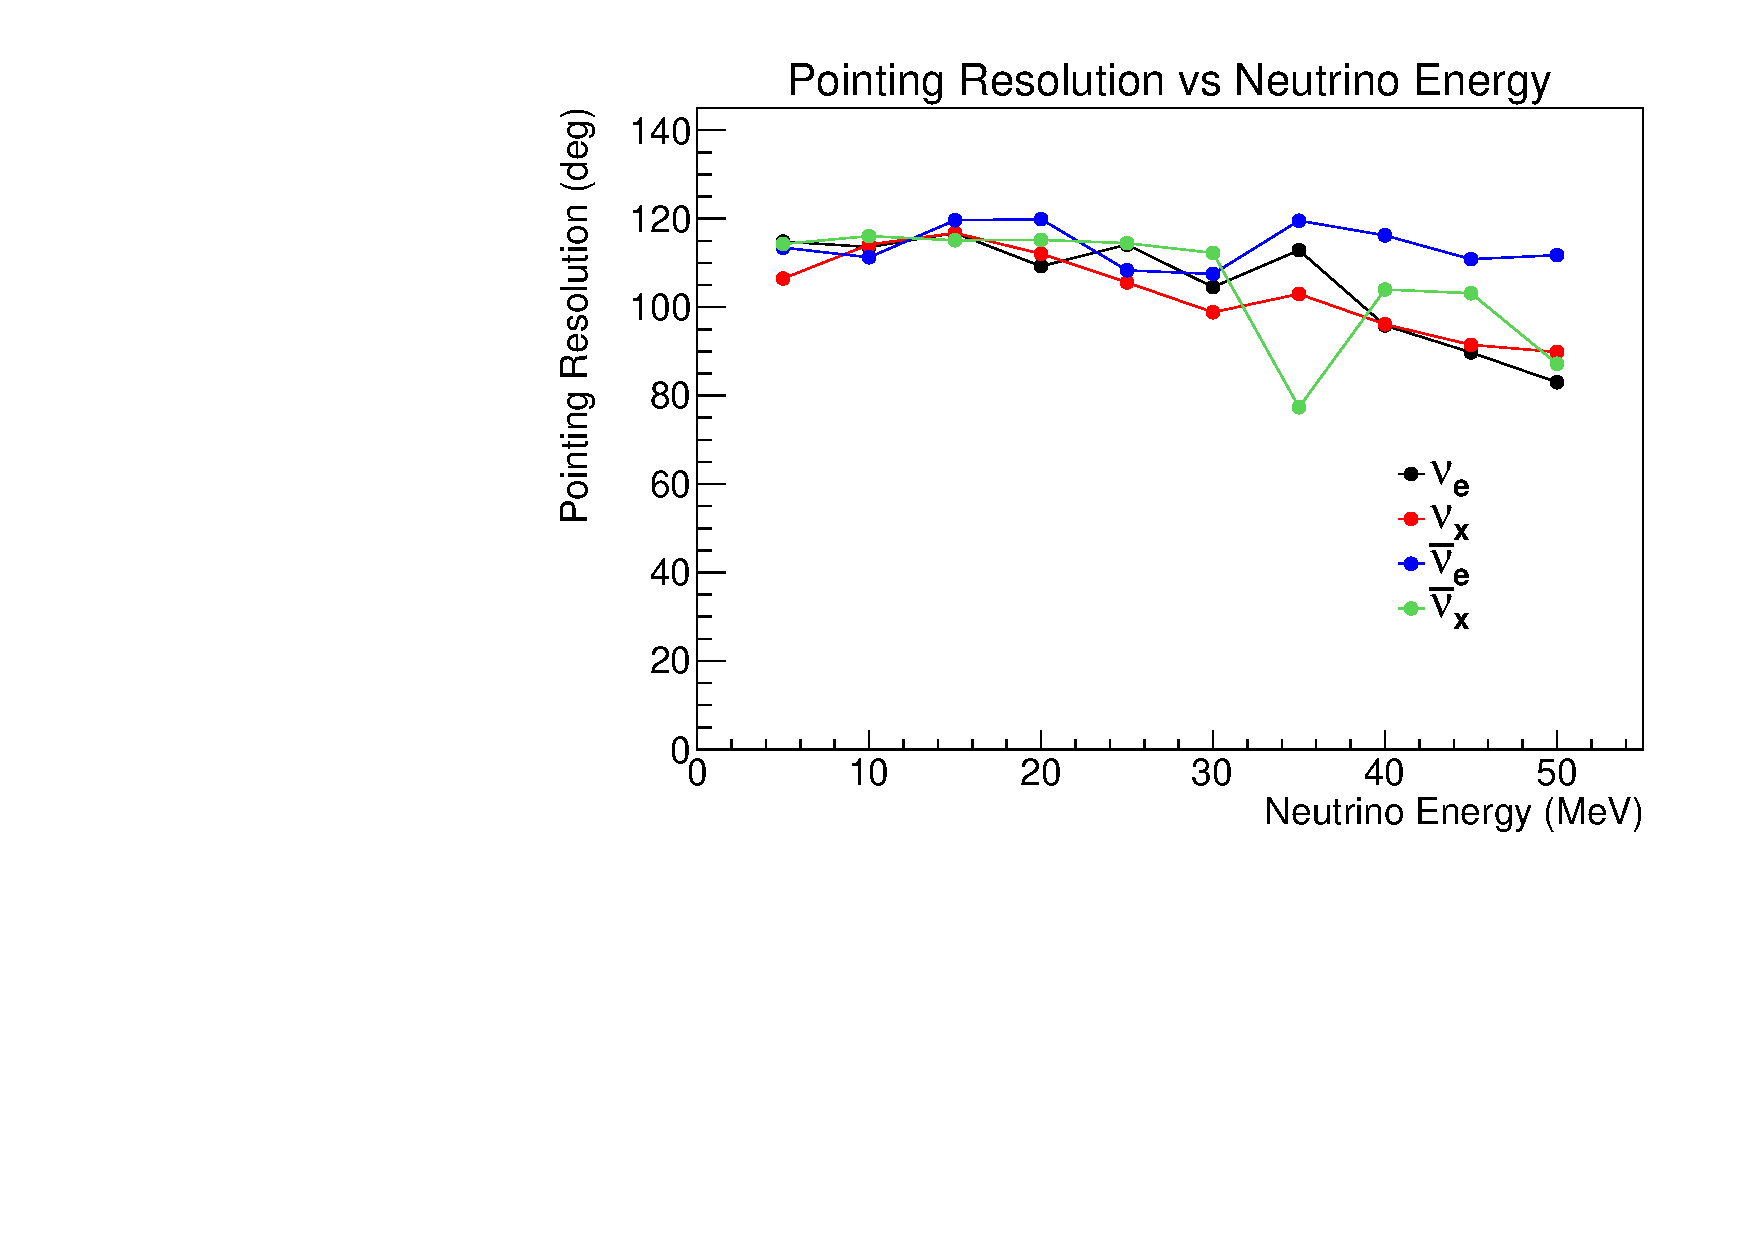
\includegraphics[width=0.4\textwidth]{pointres_vs_energy_ES_reco_dflip.pdf}
\end{dunefigure}


The pointing resolution of the reconstructed electron direction with
respect to the true neutrino direction, defined as the angle at which
68\% of angular differences are closer to truth, is plotted in
Figure~\ref{fig:ESpointres} on the right.
The absolute values of cosines of the
angular differences are used, which does not capture the head-tail
directional ambiguity of the electron track.
This pointing resolution is a result of both the neutrino-electron
angle spread, electron scattering and the error in reconstruction.  The left plot shows the
pointing resolution for electrons only, and the effect of a head-tail disambiguation
using bremsstrahlung directionality (``daughter flipping'').  Work is
continuing to improve the directional disambiguation algorithm,
including use of increased multiple
scattering towards the end of a track.

\begin{dunefigure}[Pointing for full supernova]{fig:fullSN}{Left: Log
    likelihood values as a function of direction for a 260-ES-event
    supernova sample.  Right:Distribution of angular differences for
    directions to 260-ES-event supernovae using a maximum likelihood
    method.}
  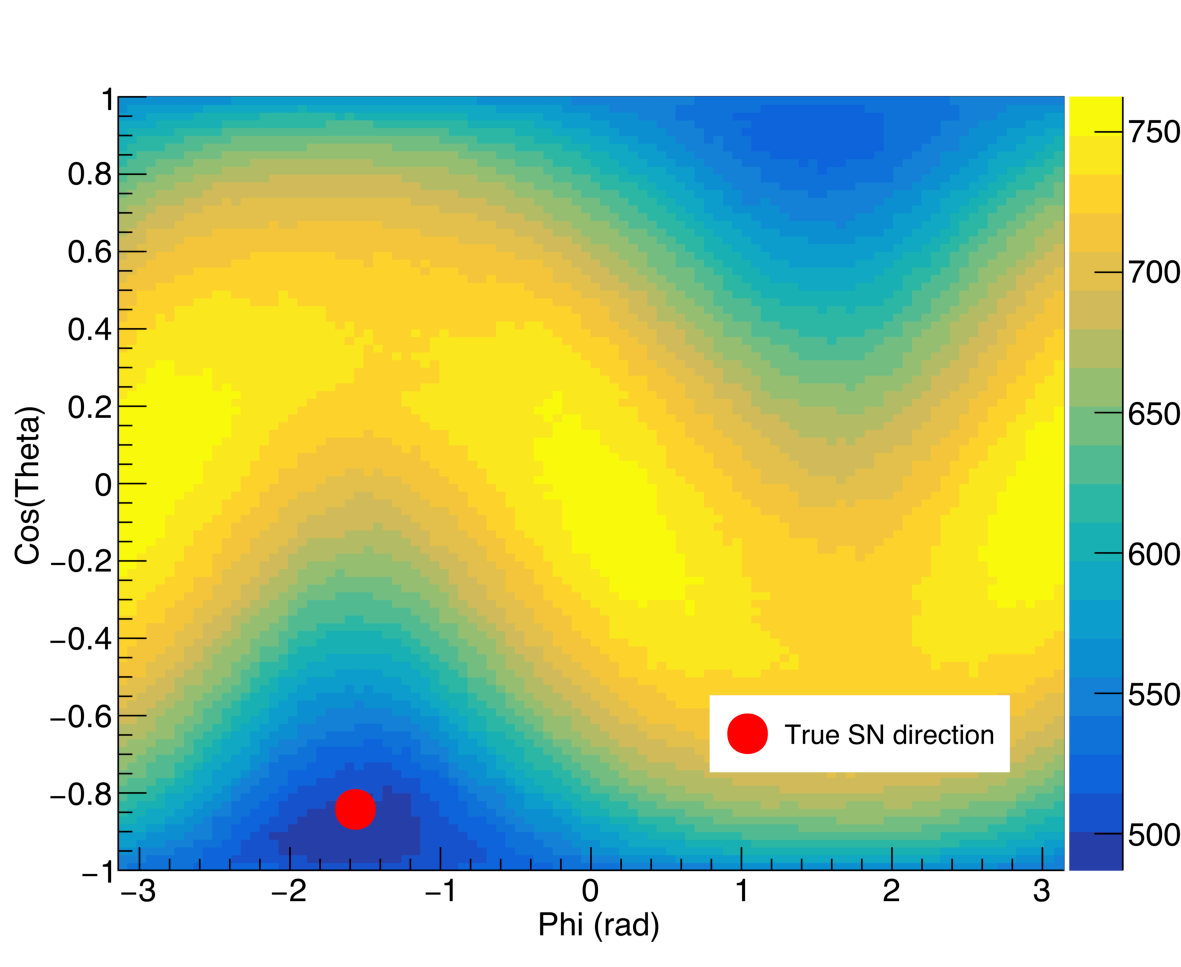
\includegraphics[width=0.44\textwidth]{LLH_15_true.pdf}
  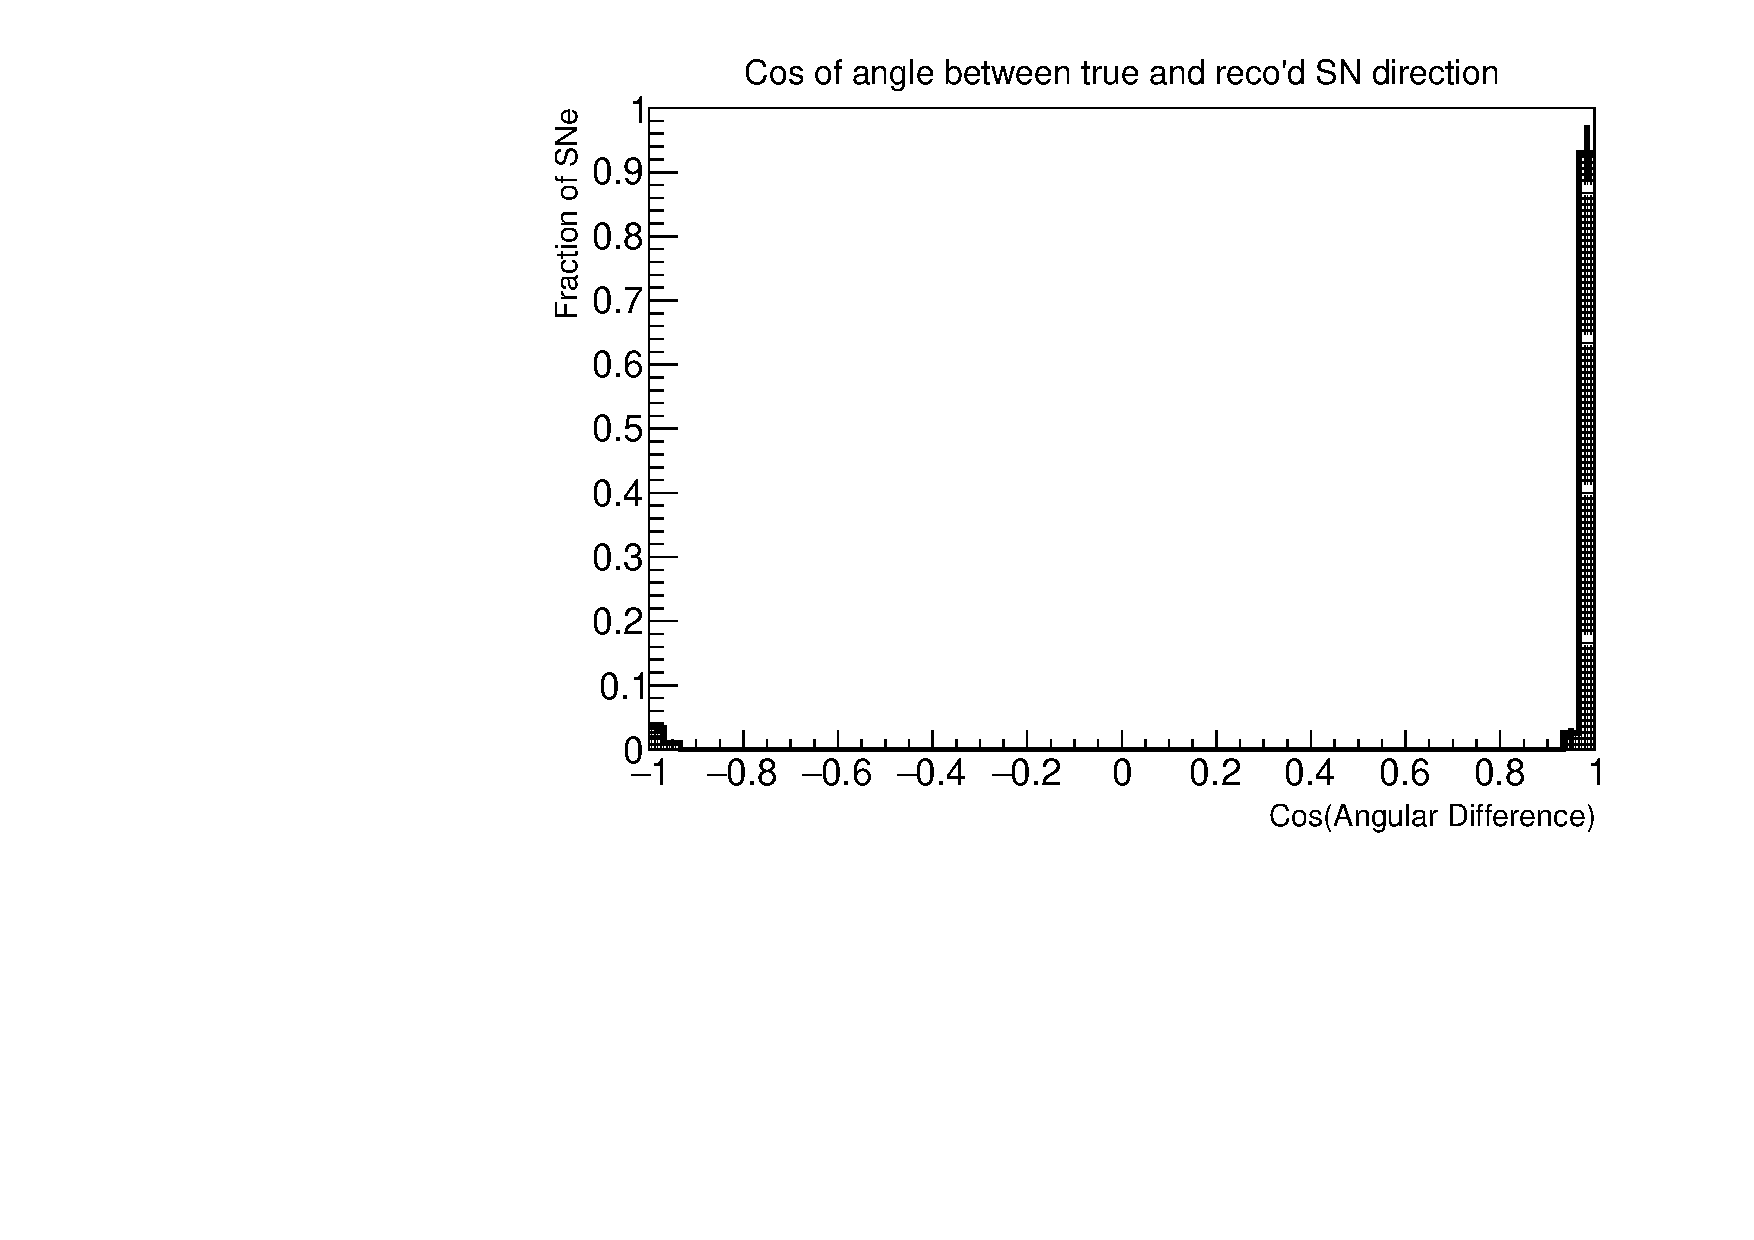
\includegraphics[width=0.44\textwidth]{costheta_SN_llhminbin_finebins.pdf}
\end{dunefigure}

If the direction can be disambiguated for $>$50\% of the individual elastic
scatters, the overall direction to the supernova can be disambuiguated
with sufficient statistics.  Since the elastic scattering angular
distribution depends on event energy, we can also make use of measured
electron energy to improve the pointing from an ensemble of events.
We employ a maximum likelihood algorithm to estimate the overall
pointing resolution to a supernova, given a mean of 260
neutrino-electron elastic scatters at 10~kpc.  Using five energy bins
in the likelihood, the results are shown in
Figure~\ref{fig:fullSN}.  Overall resolution is about 9 degrees.  This result assumes perfect selection of
elastic scatters from other interaction channels.  The dominant
$\nu_e$CC interaction channel has a weak anisotropy; additional
channels will be added to the sample and likelihood for further studies.


% \begin{dunefigure}[Pointing for full
%   supernova]{fig:SNcostheta}{Cosines of angular differences for 500
%     260-event supernova distributions of elastic scattering events,
%     after supernova ``flipping''.}
% %  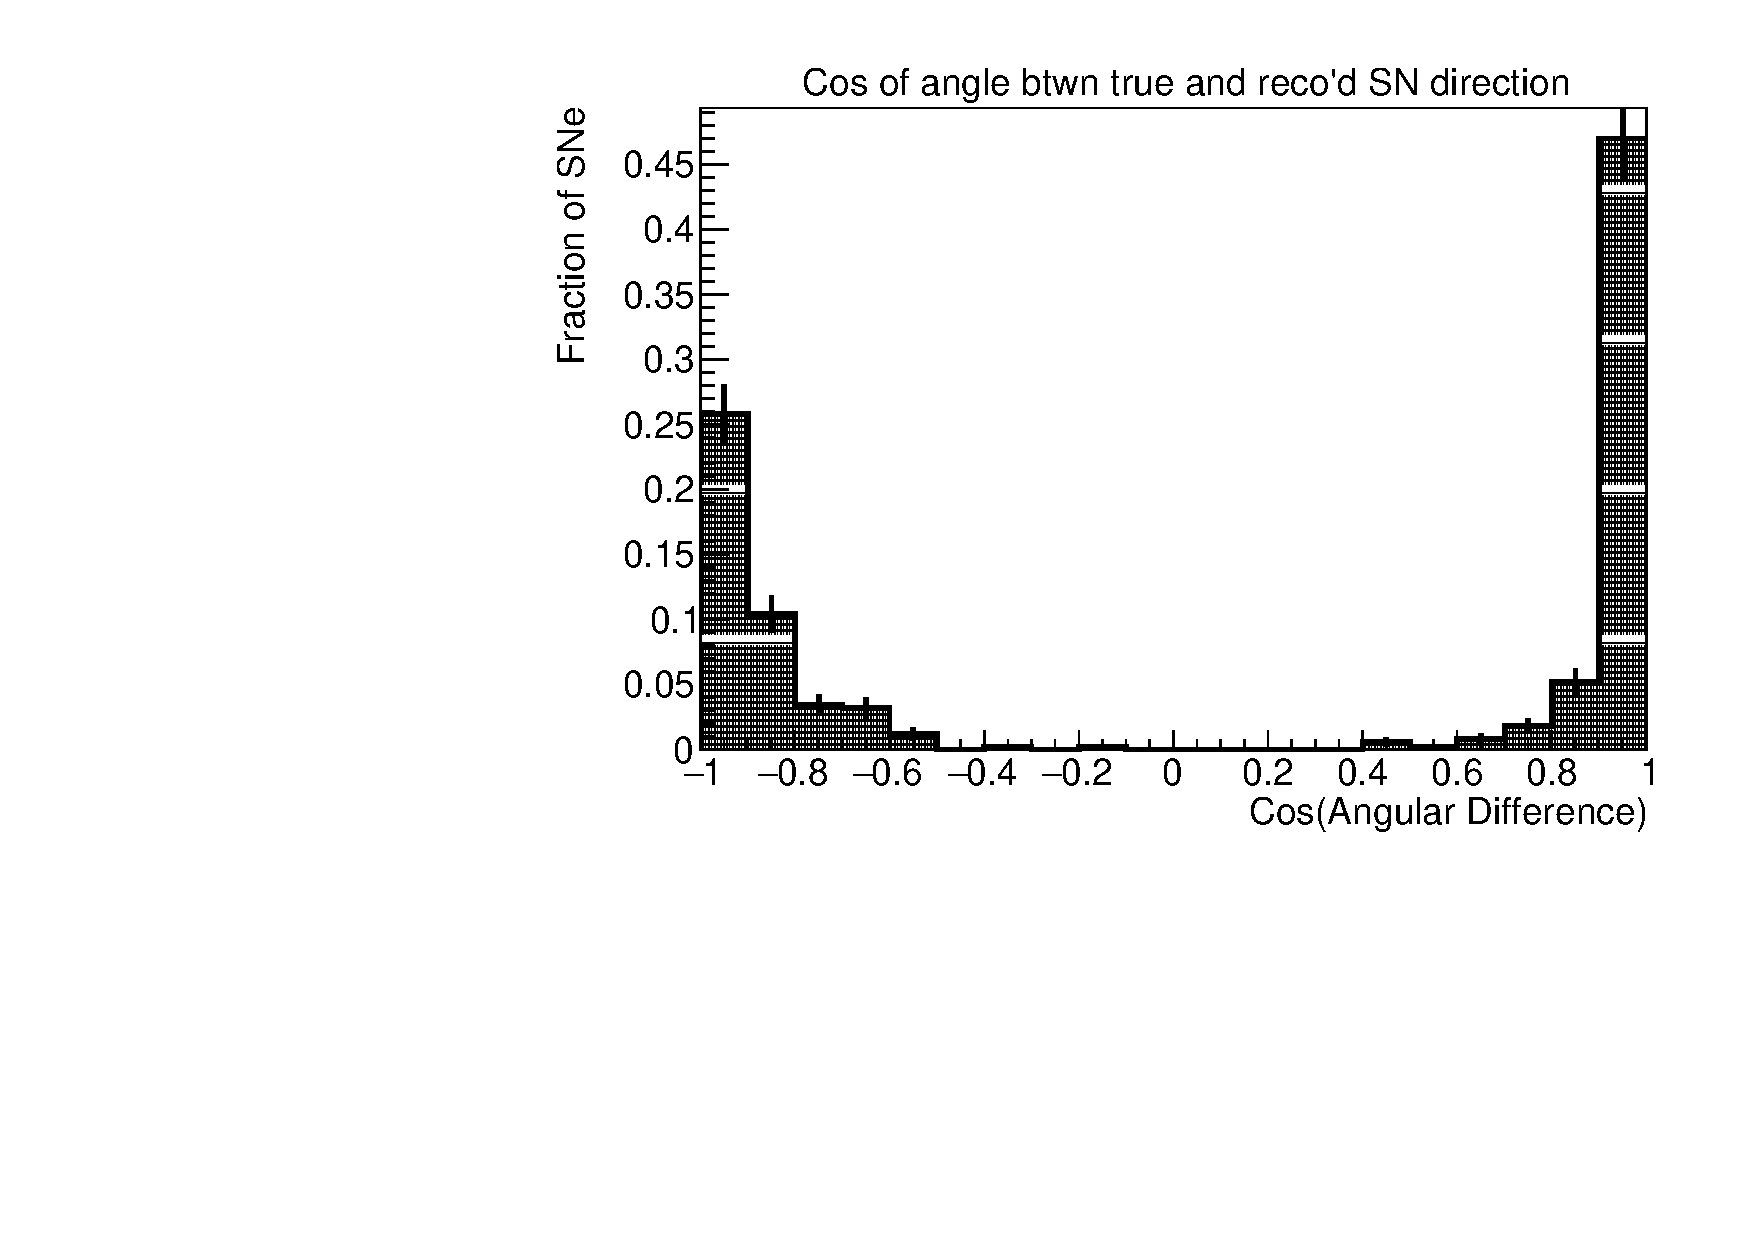
\includegraphics[width=0.6\textwidth]{costheta_SN_PMdQdx.pdf}
%   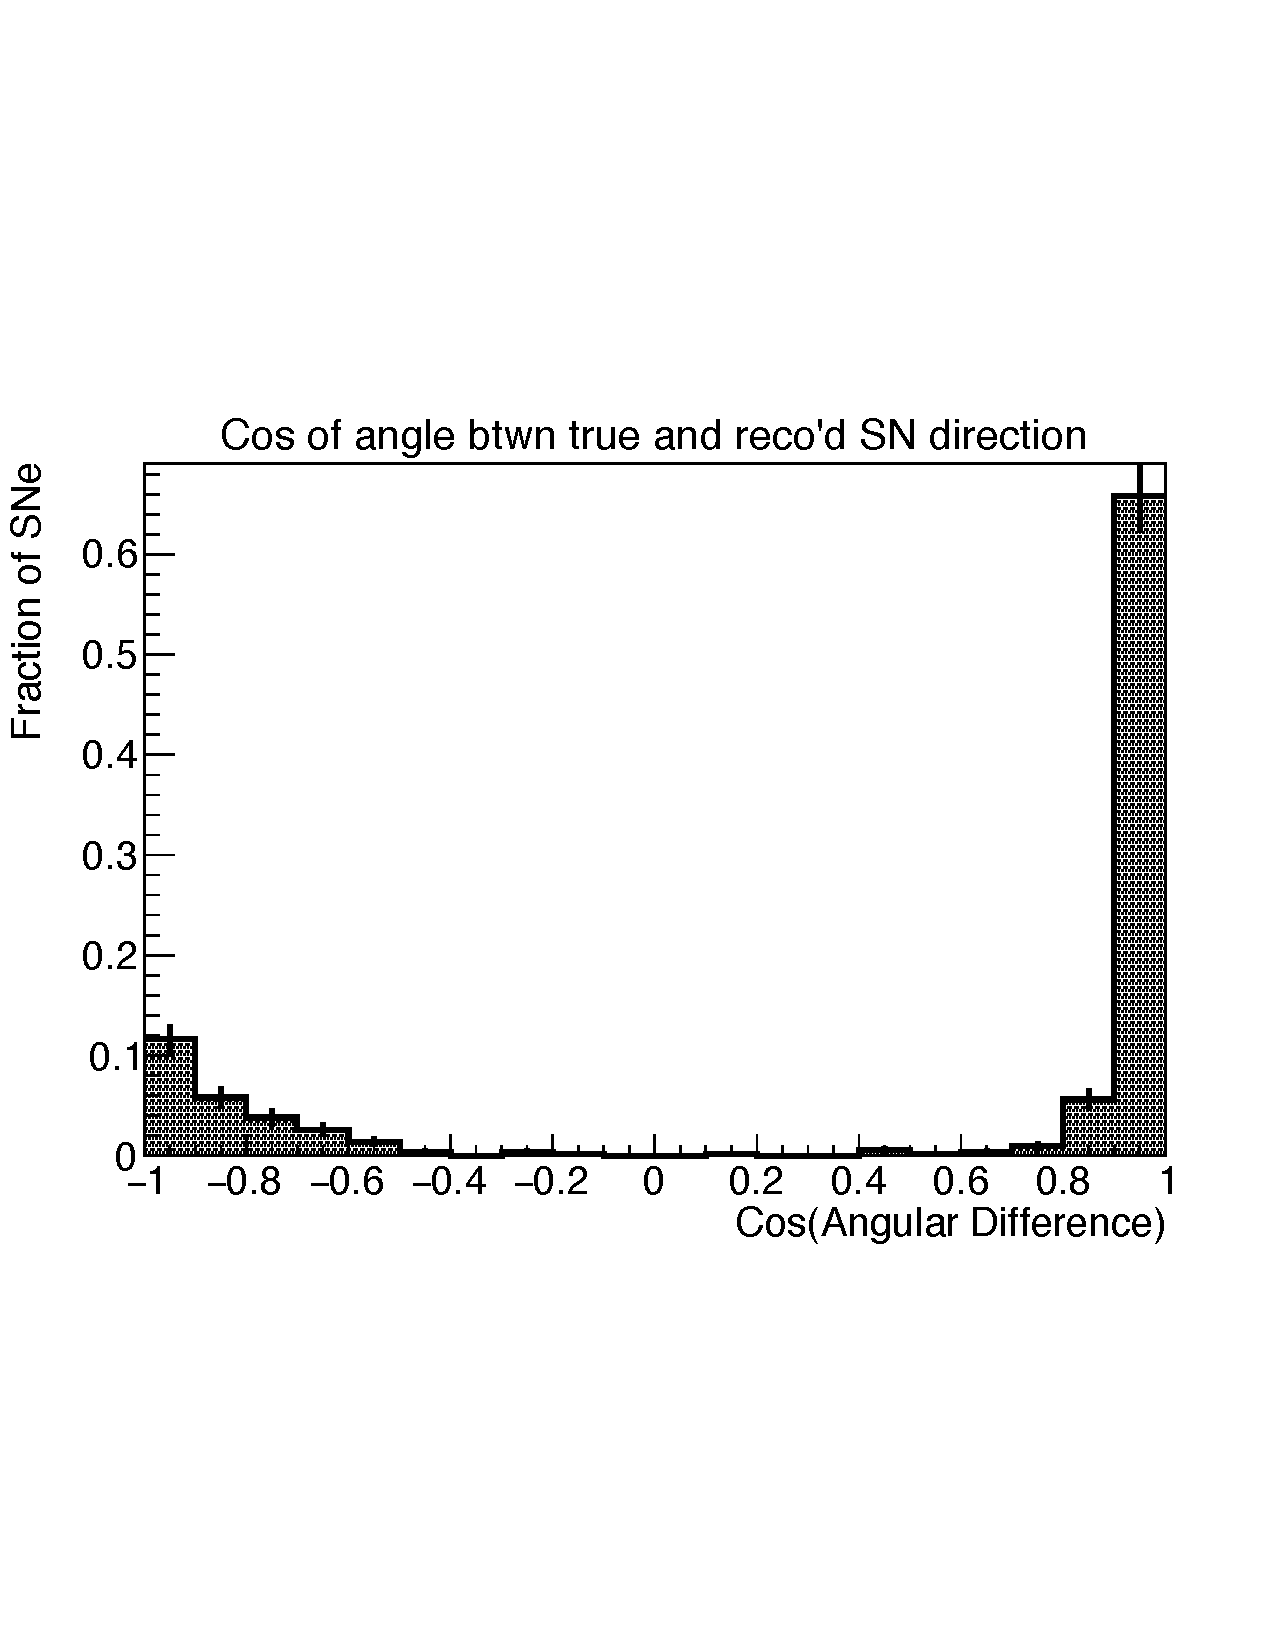
\includegraphics[width=0.6\textwidth]{costheta_SN_dflip.pdf}
% \end{dunefigure}



% In a supernova neutrino burst with many elastic scattering events from neutrinos in the same direction, however, the average direction of electrons could be an accurate estimation of the supernova direction, depending on the number of events and pointing accuracy for single electrons.
% %500 samples of elastic scattering events, with 260 events per supernova (the number of elastic scattering events expected for a supernova at a distance of 10~kpc in the GKVM model in a 40~kton fiducial volume liquid argon detector~\cite{SNOwGLoBES}), following a supernova distribution of neutrino flavor and energy (Figure~\ref{fig:SNenergyflavor}), were simulated in LArSoft version 07\_05\_00 and reconstructed uniformly in 1x2x6 far detector geometry.
% The reconstructed electron directions for each simulated supernova,
% representing 260 events corresponding to the approximate expectation
% for \dword{es} events at 10 kc, are plotted in a 2-dimensional histogram, and
% the center of the maximum bin is used as the reconstructed supernova
% direction. An example is shown in Figure~\ref{fig:recodir}, with the
% reconstructed supernova direction marked, and the true supernova
% direction marked as well for comparison.
% %In this example, the
% %reconstructed supernova direction is quite accurate. Cosines of the
% %angular differences between the reconstructed supernova directions and
% %the true neutrino directions are calculated and plotted in
% %Figure~\ref{fig:SNcostheta}.
% %, and the absolute values of those values
% %are plotted in Figure~\ref{fig:SNabscostheta}.
% %These were used to obtain the overall supernova pointing resolutions, shown in Table~\ref{tab:SNpointres}.
% For a supernova with multiple elastic scattering events, the
% directional ambiguity discussed above causes there to be two clusters
% of directions, where one cluster is around the true supernova
% direction and the other is around 180$^{\circ}$ from the true
% supernova direction.
% % as seen in Figure~\ref{fig:recodir}.
% If the direction can be determined correctly more than 50\% of the
% time, then the tracks that were reconstructed backwards can be
% corrected (``flipped''). For each track, the directions starting from
% each end of the track are compared to the reconstructed supernova
% direction, and whichever is closer is assumed to be the correct
% electron direction.  Figure~\ref{fig:recodir} shows the result before
% and after flipping.
% %Figure~\ref{fig:recodirSNflip} is the same
% %simulated supernova shown in Figure~\ref{fig:recodir} after flipping
% %based on the supernova direction was done.
% Overall, the directional
% ambiguity can be reduced using a statistical sample.
% %There are very few counts near 180$^{\circ}$ from the true supernova
% %direction, and more counts closer to the true supernova direction.
% The cosines of angular differences are plotted in
% Figure~\ref{fig:SNcostheta}.    Overall pointing resolution is about 31$^\circ$.
% %and the absolute values of those values were plotted in
% %Figure~\ref{fig:SNabscosthetaSNflip}.
% %The pointing resolutions for supernovae are summarized in in Table~\ref{tab:SNpointres}.



% \begin{table}[ht]
% \centering
% Pointing Resolution for Expected Supernova Elastic Scattering Signal \\
% \begin{tabular}{| c | c | c |}
% \hline
%  & True values & Absolute values \\
% \hline
% No supernova direction flipping & 147.2$^{\circ}$ & 25.0$^{\circ}$ \\
% \hline
% Supernova direction flipping & 150.2$^{\circ}$ & 23.7$^{\circ}$ \\
% \hline
% Daughter flipping and supernova direction flipping & 31$^{\circ}$ & \\
% \hline
% \end{tabular}
% \caption{\label{tab:SNpointres}Pointing resolution for elastic scattering events following 10~kpc supernova flavor and energy distribution, with and without supernova direction flipping and daughter flipping, using true cosines of angular differences and absolute values of those values.}
% \end{table}



\section{Astrophysics of Core Collapse}
\label{sec:physics-snblowe-astrophysics}


A number of astrophysical phenomena associated with supernovae are expected to be observable
in the supernova neutrino signal, providing a remarkable window into the event.  In particular, the supernova explosion mechanism, which in the current paradigm involves energy deposition via neutrinos, is still not well understood, and the neutrinos themselves will bring the insight needed to confirm or refute the paradigm.

There are many other examples of astrophysical observables.
\begin{itemize}
\item The initial burst, primarily composed of $\nu_e$ and called the
  ``neutronization'' or ``breakout''
  burst, 
  represents only a small component of the total signal.  However,
  oscillation effects can manifest themselves in an observable manner
  in this burst, and flavor transformations can be modified by the
  ``halo'' of neutrinos generated in the supernova envelope by
  scattering~\cite{Cherry:2013mv}.
\item The formation of a black hole would cause a sharp signal cutoff
  (e.g.,~\cite{Beacom:2000qy,Fischer:2008rh}).
\item Shock wave effects (e.g.,~\cite{Schirato:2002tg}) would cause a
  time-dependent change in flavor and spectral composition as the
  shock wave propagates.
\item The standing accretion shock instability
  (SASI)~\cite{Hanke:2011jf,Hanke:2013ena}, a ``sloshing'' mode
  predicted by three-dimensional neutrino-hydrodynamics simulations of
  supernova cores, would give an oscillatory flavor-dependent
  modulation of the flux.
\item Turbulence effects~\cite{Friedland:2006ta,Lund:2013uta} would
  also cause flavor-dependent spectral modification as a function of
  time.
%  \item Strange star formation
\end{itemize}

Observation of a supernova neutrino burst in coincidence with gravitational waves (which would also be prompt, and could indeed provide a time reference for a a time-of-flight analysis) would be especially interesting~\cite{Arnaud:2003zr,Ott:2012jq, Mueller:2012sv, Nishizawa:2014zna}.

The supernova neutrino burst is prompt with respect to the
electromagnetic signal and therefore can be exploited to provide an
early warning to astronomers~\cite{Antonioli:2004zb,Scholberg:2008fa}.  
Additionally, a liquid argon signal~\cite{Bueno:2003ei} is expected to
provide some pointing information, primarily from elastic scattering
on electrons.
We note that not every core collapse will produce an observable supernova, and observation of a neutrino burst in the absence of an electromagnetic event would be very interesting. 

Even non-observation of a burst, or non-observation of
a $\nu_e$ component of a burst in the presence of supernovae (or other
astrophysical events) observed in electromagnetic or gravitational
wave channels, would still provide valuable information about the
nature of the sources.  Further, a long-timescale, sensitive search
yielding no bursts will also provide limits on the rate of
core-collapse supernovae.

We note that the better one can understand the astrophysical nature of core-collapse supernovae, the easier it will be to extract information about particle physics.  DUNE's capability to characterize the $\nu_e$ component of the signal is unique and critical.

\subsection{Supernova Spectral Parameter Fits}

% From Erin

We have investigated how well it will be possible to fit to the supernova
spectral parameters, to determine, for example, the $\epsilon$
parameter related to the total binding energy release of the supernova.  We 
use  \dword{snowglobes} to model signals described by the pinched-thermal form.

We have developed a
forward fitting algorithm requiring a  \dword{snowglobes} binned energy
spectrum for a supernova at a given distance and a ``true" set of
pinched-thermal parameters $(\alpha^0, \langle E_\nu \rangle^0,
\varepsilon^0)$. As an example, we define the true parameter values as
$(\alpha^0, \langle E_\nu \rangle^0, \varepsilon^0) = (2.5, 9.5,
5\times 10^{52})$, with $\varepsilon$ in ergs/second, assumed
integrated over a ten-second burst.
We focus on the electron neutrino flux. The algorithm uses this
spectrum as a ``test spectrum" to compare against a grid of energy
spectra generated with many different combinations of $(\alpha,
\langle E_\nu \rangle, \varepsilon)$. To quantify these comparisons,
the algorithm employs $\chi^2$ minimization technique to find the
best-fit spectrum.

% s and uses the following definition of the $\chi^2$ function:

% \begin{equation}
%     \chi^2(x) = \sum_{i=1}^{N_b} \frac{\big[N_i(\alpha, \langle E_\nu \rangle, \varepsilon) - N_i(\alpha^0, \langle E_\nu \rangle^0, \varepsilon^0)\big]^2}{\sigma_i^2(x)}
%     \label{chi2function}
% \end{equation}

% Equation \ref{chi2function} contains the following variables:
% \begin{itemize}
%     \setlength\itemsep{0.1em}
%     \item $N_b$ is the number of bins for the energy spectra.
%     \item $N_{i}$ is the number of events in bin $i$.
%     \item $\sigma_i$ is the uncertainty of the contents in bin $i$. This technical note uses Poisson uncertainties.
%     \item $(\alpha, \langle E_\nu \rangle, \varepsilon)$ are the set of model parameters used to generate an energy spectrum in the grid.
%     \item $(\alpha^0, \langle E_\nu \rangle^0, \varepsilon^0)$ are the model parameters used to generate the test spectrum.
% \end{itemize}

% Fig. \ref{exampleFitting} shows an example of $\chi^2$ minimization of a test spectrum against an arbitrary grid element. The forward fitting algorithm implements Eq. \ref{chi2function} to compare the test spectrum to all elements in the grid, and the smallest $\chi^2$ corresponds to the grid element that best fits the test spectrum.

% \begin{dunefigure}[Test spectrum for SN parameter fitting]{exampleFitting}{Event rates calculated using SNOwGLoBES for a test spectrum and an example grid element.}
% 	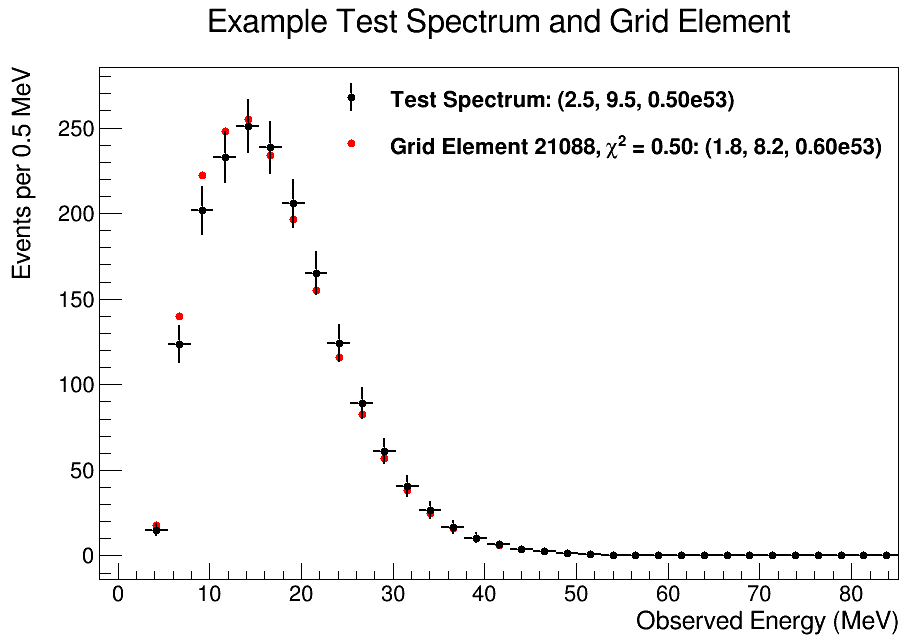
\includegraphics[scale = 0.25]{SuperimposedTestSpectrumGridElements3.png}
% \end{dunefigure}

A test spectrum input into the forward fitting algorithm produces a set of $\chi^2$ values for every element in a grid. While the smallest $\chi^2$ value determines the best fit to the test spectrum, there exists other grid elements that reasonably fit the test spectrum according to their $\chi^2$ values. The collection of these grid elements help determine the parameter measurement uncertainty, and we represent this using ``sensitivity regions" in 2D spectral parameter space. We can use three sets of 2D parameter spaces: $(\langle E_\nu \rangle, \alpha)$, $(\langle E_\nu \rangle, \varepsilon)$, and $(\alpha, \varepsilon)$.

One ``point" in 2D parameter space encompasses several grid elements,
e.g., the $(\langle E_\nu \rangle, \alpha)$ space contains different
$\varepsilon$ values for a given values of $\langle E_\nu \rangle$ and
$\alpha$. To determine the $\chi^2$ value, we profile over
$\varepsilon$ to select the grid element with the smallest
$\chi^2$. We determine the sensitivity regions by placing a cut of
$\chi^2 = 6.25$ corresponding to a 90\% coverage probability for three
free parameters.
%\cite{Tanabashi:2018oca} ???\cite{pdg} 

\begin{dunefigure}[Example of distance
  effect]{exampleAsimovDistance}{Sensitivity regions generated using
    the Asimov study in $(\langle E_\nu \rangle, \varepsilon)$ space
    for three different supernova distances.  \dword{snowglobes} used a
    smearing matrix with 15\% Gaussian resolution, a cross section
    model from \dword{marley}, and a step efficiency function with a 5 MeV
    detected energy threshold.}
	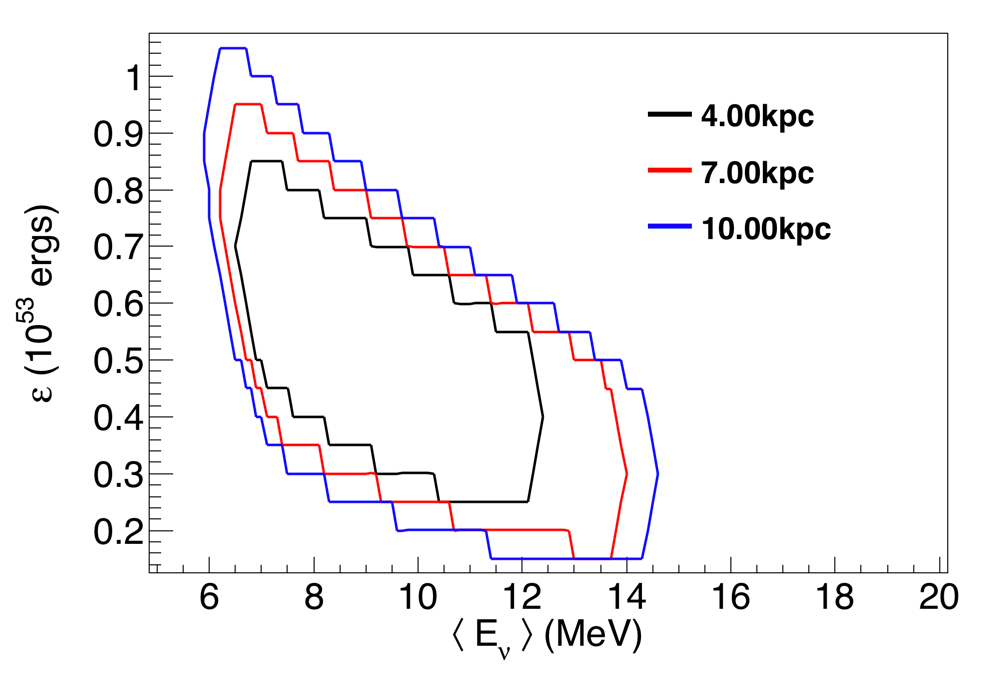
\includegraphics[scale = 0.37]{LuminosityVsMeanE_SensitivityRegions.png}
  \end{dunefigure}


  
%Comparing sensitivity regions corresponding to different combinations of test spectrum and grid resolution aids in understanding how regions shift and grow in 2D parameter space. We can also discern features and patterns present in the 2D contour area plots. Fig. \ref{ResolutionStudy_SensitivityRegions} shows sensitivity regions for different combinations of test spectrum and grid resolution. The figure shows how the regions change as the assumptions change, and we also observe how the best-fit parameters shift in 2D parameter space. These shifts represent the biases on the best-fit parameters.

% \begin{dunefigure}[Resolution study]{ResolutionStudy_SensitivityRegions}{Sensitivity regions for a test spectrum produced with 30\% resolution as input into four different grids: a grid produced with resolution values of 0\% (black), 10\% (red), 20\% (green), and 30\% (blue). The best-fit parameters (stars) are also plotted. The contour areas increase as the grid resolution increases because more grid elements reasonably match the test spectrum as the assumed and true resolutions differ less.}
% 	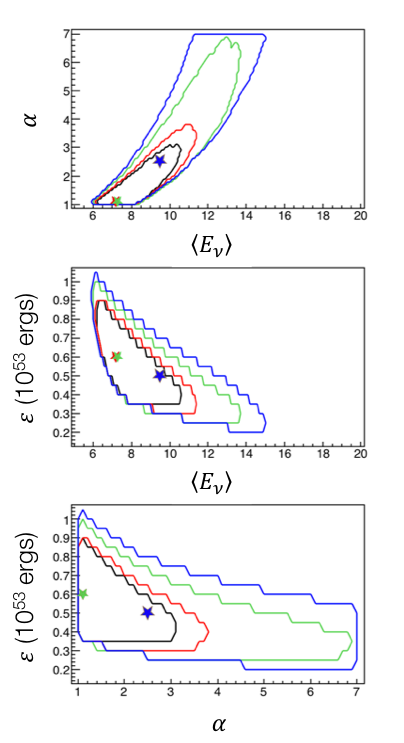
\includegraphics[scale = 1.1]{ResolutionStudy_SensitivityRegions.png}
% \end{dunefigure}



  We have used this method to study the effect of detector parameters,
  and required \textit{knowledge} of detector parameters, on ability
  to extract the flux parameters. While the size of the sensitivity
  regions is highly dependent on statistics (and hence distance), we
  find biases in the best-fit physics parameters
  if assumed understanding of detector parameters such as
 energy resolution, energy threshold, and energy scale does not match
 the truth.  We have
also studied the effect of imperfect knowledge of the $\nu_e$ cross
section on argon.  The results of these studies are extensive and
documented in Ref.~\cite{docdb14068}.
  
% Citing tech note OK??  How?



\section{Neutrino Physics and Other Particle Physics}
\label{sec:physics-snblowe-neutrino-physics}

A core-collapse supernova is essentially a gravity-powered neutrino bomb: the energy of the collapse is initially stored in the Fermi seas of electrons and neutrinos and then gradually leaked out by neutrino diffusion. The key property of neutrinos that makes them play such a dominant role in the supernova dynamics is the feebleness of their interactions. It then follows that should there be new light ($< 100$ MeV) particles with even weaker interactions, they could alter the energy transport process and the resulting evolution of the nascent proto-neutron star. Moreover, additional interactions or properties of neutrinos could also be manifested in this way. 

Thus, a core-collapse supernova can therefore be thought of as an extremely hermetic system, which can be used to search for numerous types of new physics (e.g.,~\cite{Schramm:1990pf,Raffelt:1999tx}). The list includes various Goldstone bosons (e.g., Majorons), neutrino magnetic moments, new gauge bosons (``dark photons''), ``unparticles'', and extra-dimensional gauge bosons. The existing data from SN1987A already provides significant constraints on these scenarios, by confirming the basic energy balance of the explosion. At the same time, more precision is highly desirable and should be provided with the next galactic supernova. 

% \begin{dunefigure}[Simulated cooling curves from the Garching light progenitor model]{coolingcurves}{ Average $\nu_{e}$ energy from a simulated fit to the oscillated fluxes predicted by the Garching 1D model with a light (10.8 $M_{\odot}$) progenitor. Our oscillation calculations included full multi-angle treatment of collective evolution, for two
% different mass hierarchy assumptions. The predicted events were then smeared with SNOwGLoBES and fit with pinched-thermal spectrum as a function of time (assuming a supernova at 10 kpc and a 34 kt LAr detector). The bands represent $1\sigma$ error bars from the fit (assuming only statistical uncertainties). The solid black line is the true
% $\langle E_{\nu} \rangle$ for the unoscillated spectrum. Clearly, the rate of energy escape from the proto-neutron star can be gleaned by tracking $\nu_{e}$ spectra as a function of time.}
% %\includegraphics[width=0.9\textwidth]{timedep.pdf}
% \end{dunefigure}



Such energy-loss-based analysis will make use of two types of information. First, the total energy of the emitted neutrinos should be compared with the expected release in the gravitational collapse.  Note that measurements of all flavors, including $\nu_e$, are needed for the best estimate of the energy release.
Second, the rate of cooling of the protoneutron state should be measured and compared with what is expected from diffusion of the standard neutrinos.% This requires comparing one-second-interval time-integrated spectra at successive times as illustrated in Figure~\ref{fig:coolingcurves}. 

Because DUNE is mostly sensitive to $\nu_e$, complementary data from
water Cherenkov detector and scintillator for the measurement of
$\bar\nu_{e}$ and a careful analysis of the oscillation pattern (see
below) will enable inference of the fluxes of $\mu$ and $\tau$
flavors. As for measuring the energy loss rate, it will require
sufficient statistics at late times.
%and, once again, understanding the oscillation dynamics, as is clear in Figure~\ref{fig:coolingcurves} where oscillated and unoscillated cases are shown.

The flavor oscillation physics and its signatures are a major part of
the physics program. Compared to the well-understood case of solar
neutrinos, in a supernova, neutrino flavor transformations are much
more involved. For supernovae, there are both neutrinos and antineutrinos, and
two mass splittings---``solar" and ``atmospheric" to worry about.
While flavor transitions can be reasonably well understood during 
early periods of the neutrino emission as standard \dword{msw} 
transitions in the varying density profile of the overlying material, during
later periods the physics of the transformations is significantly richer.
For example, several seconds after the onset of the explosion, the
flavor conversion probability is affected by the expanding shock front
and the turbulent region behind it. The conversion process in such a
stochastic profile is qualitatively different from the adiabatic \dword{msw}
effect in the smooth, fixed density profile of the Sun . 

Even more complexity is brought about by the coherent scattering of neutrinos off each other. This neutrino ``self-refraction'' 
 results in highly nontrivial flavor transformations close to the neutrinosphere, typically within a few hundred kilometers from the center, where the density of streaming neutrinos is very high. Since the evolving flavor composition of the neutrino flux feeds back into the oscillation Hamiltonian, the problem is \emph{nonlinear}. Furthermore, as the interactions couple neutrinos and antineutrinos of different flavors and energies, the oscillations are characterized by \emph{collective} modes.    This leads to very rich physics that has been the subject of intense interest over the last decade and a voluminous literature exists exploring these collective phenomena,
e.g.,~\cite{Duan:2005cp,Fogli:2007bk,Raffelt:2007cb,Raffelt:2007xt,EstebanPretel:2008ni,Duan:2009cd,Dasgupta:2009mg,Duan:2010bg,Duan:2010bf,Wu:2014kaa}.  This is an active theoretical field and the effects are not yet fully understood. A supernova burst is the only opportunity to study neutrino-neutrino interactions experimentally.

% \begin{dunefigure}[Simulated cooling curves from the Garching light progenitor model]{shockandcollective}{ A simulation of the effects of collective oscillations alone (left panel) and of collective oscillations plus the shock front (right panel). Solid lines are unoscillated $\nu_e$ (green, cooler) and $\nu_x$ (blue, hotter) and filled curve is after collective oscillations. (Flux in arbitrary units)}
% %\includegraphics[width=0.9\textwidth]{shockandcollective.pdf}
% \end{dunefigure}

One may wonder whether all this complexity will impede the extraction
of useful information from the future signal. In fact, the opposite is
true: the new effects can \emph{imprint} information about the inner
workings of the explosion on the signal. The oscillations can modulate
the characteristics of the signal (both event rates and spectra as a
function of time).
%as seen in Figure~\ref{fig:coolingcurves}.
Moreover, the oscillations can imprint \emph{non-thermal} features on the energy spectra, potentially making it possible to disentangle the effects of flavor transformations and the physics of neutrino spectra formation. This in turn should help us learn about the development of the explosion during the crucial first 10 seconds.   It is important to note that the features depend on the unknown mass hierarchy, and so can potentially tell us what the hierarchy is.

% An illustration is provided in Figure~\ref{fig:shockandcollective}. The role of the collective oscillations in this case is to almost completely permute the original $\nu_{e}$ and $\nu_{\mu,\tau}$ spectra, so that the flux of observed electron neutrinos is noticeably hotter than the original one. Moreover, the shock front modulated the \dword{msw} conversion probability and imprints a nonthermal ``step'' in the spectrum. Below this step, the swap between the original $\nu_{e}$ and $\nu_{\mu,\tau}$ spectra is only partial. As the shock expands, the feature moves to higher energies, creating a ``smoking-gun'' signature that exists only in the neutrino channel. 

In the following, we examine quantitatively two examples of particle
physics that can be accessed: neutrino mass hierarchy and Lorentz
invariance violation.
%\textit{An additional section on collective
%  oscillation observability will be added if the study is completed in
% the next month.}


\subsection{Neutrino Mass Hierarchy}\label{sec:mh}


As described above, flavor transitions
%\footnote{Smirnov comment}
in the supernova can be fairly complex, and the rich phenomenology is
at this time still under active investigation.  The neutrino mass
hierarchy affects the specific flavor composition in multiple ways
during the different eras of neutrino emission.  
References~\cite{Mirizzi:2015eza,Scholberg:2017czd} survey in some detail the
multiple signatures of mass hierarchy that will imprint themselves on
the flux.  Table~\ref{tab:snmo} summarized several of them. For many of these, the $\nu_e$ component of the signal will
be critical to measure.    Some signatures of mass hierarchy are more robust than
others, in the sense that the assumptions are less subject to
theoretical uncertainties.  One of the more robust of these is the
early-time signal, including the \textit{neutronization burst}.   At
early times, the matter potential is dominant over the
neutrino-neutrino potential, which means that standard \dword{msw} effects are
in play.  In this case, for the \dword{nh}, the neutronization burst, which is
emitted as nearly pure $\nu_e$, is strongly suppressed, whereas for
the \dword{ih}, the neutronization burst is only partly suppressed.  
% Put the equation shere.
Figure~\ref{fig:early} gives an example for a specific model, but which
shows typical features.  The same \dword{msw}-dominated transitions also
affect
the subsequent rise of the signal over a fraction of a second; here
the time profile will depend on the turn-on of the non-$\nu_e$ flavors.

\begin{dunetable}[Supernova mass hierarchy
  signatures]{|c|c|c|c|c|}{tab:snmo}{Table taken from
    ~\cite{Scholberg:2017czd} qualitatively summarizing different neutrino mass hierarchy
    signatures that will manifest themselves in the supernova neutrino
  time, energy and flavor structure of the burst.}

Signature & Normal &  Inverted & Robustness & Observability\\ 

 Neutronization & \small Very suppressed & \small Suppressed & \small
 Excellent & \small Good, need $\nu_e$ \\  \colhline
% & \small suppressed & & & \\  \colhline  
Early time profile & \small Low then high & \small Flatter & \small Good,
possibly some self-interaction & \small Good \\ \colhline 
%     & \small high &  & \small possibly some& \small especially IceCube\\ 
%     &                   && \small self-interaction &\\
 %    &                   & &  \small effects & \\  \colhline
Shock wave & \small Time- & \small Time- & \small Fair,  & \small May be \\ 
        &\small dependent & \small dependent & \small entangled with & \small statistics\\ 
       &                 &                    & \small  self-interaction     &  \small limited\\ 

  & & & \small effects& \\  \colhline
   
Collective effects &\multicolumn{2}{|c|} {\small Various time- and energy-} & \small Unknown, but & \small Want all\\ 
 & \multicolumn{2}{|c|} {\small dependent signatures} & \small multiple signatures &\small flavors\\  \colhline
Earth matter & \small Wiggles in $\bar{\nu}_e$ & \small Wiggles in $\nu_e$ & \small Excellent & \small Difficult, need\\ 
& & & & \small energy resolution,\\ 
& & & &  \small Earth shadowing\\   \colhline
Type Ia &  \small Lower flux & \small Higher flux& \small Moderate & \small Need large detectors,  \\
  & & & & \small very close SN\\  \colhline

\end{dunetable}


\begin{dunefigure}[Event rates with hierarchy effects at early times]{fig:early}
{Expected event rates as a function of time for the electron-capture model in~\cite{Huedepohl:2009wh} for \SI{40}{kt} of argon during early stages of the event -- the neutronization burst and early accretion phases, for which self-induced effects are unlikely to be important.  Shown is the event rate for the unrealistic case of no flavor transitions (blue), the event rate including the effect of matter transitions for the normal (red)  and inverted (green) hierarchies.  Error bars are statistical, in unequal time bins.}
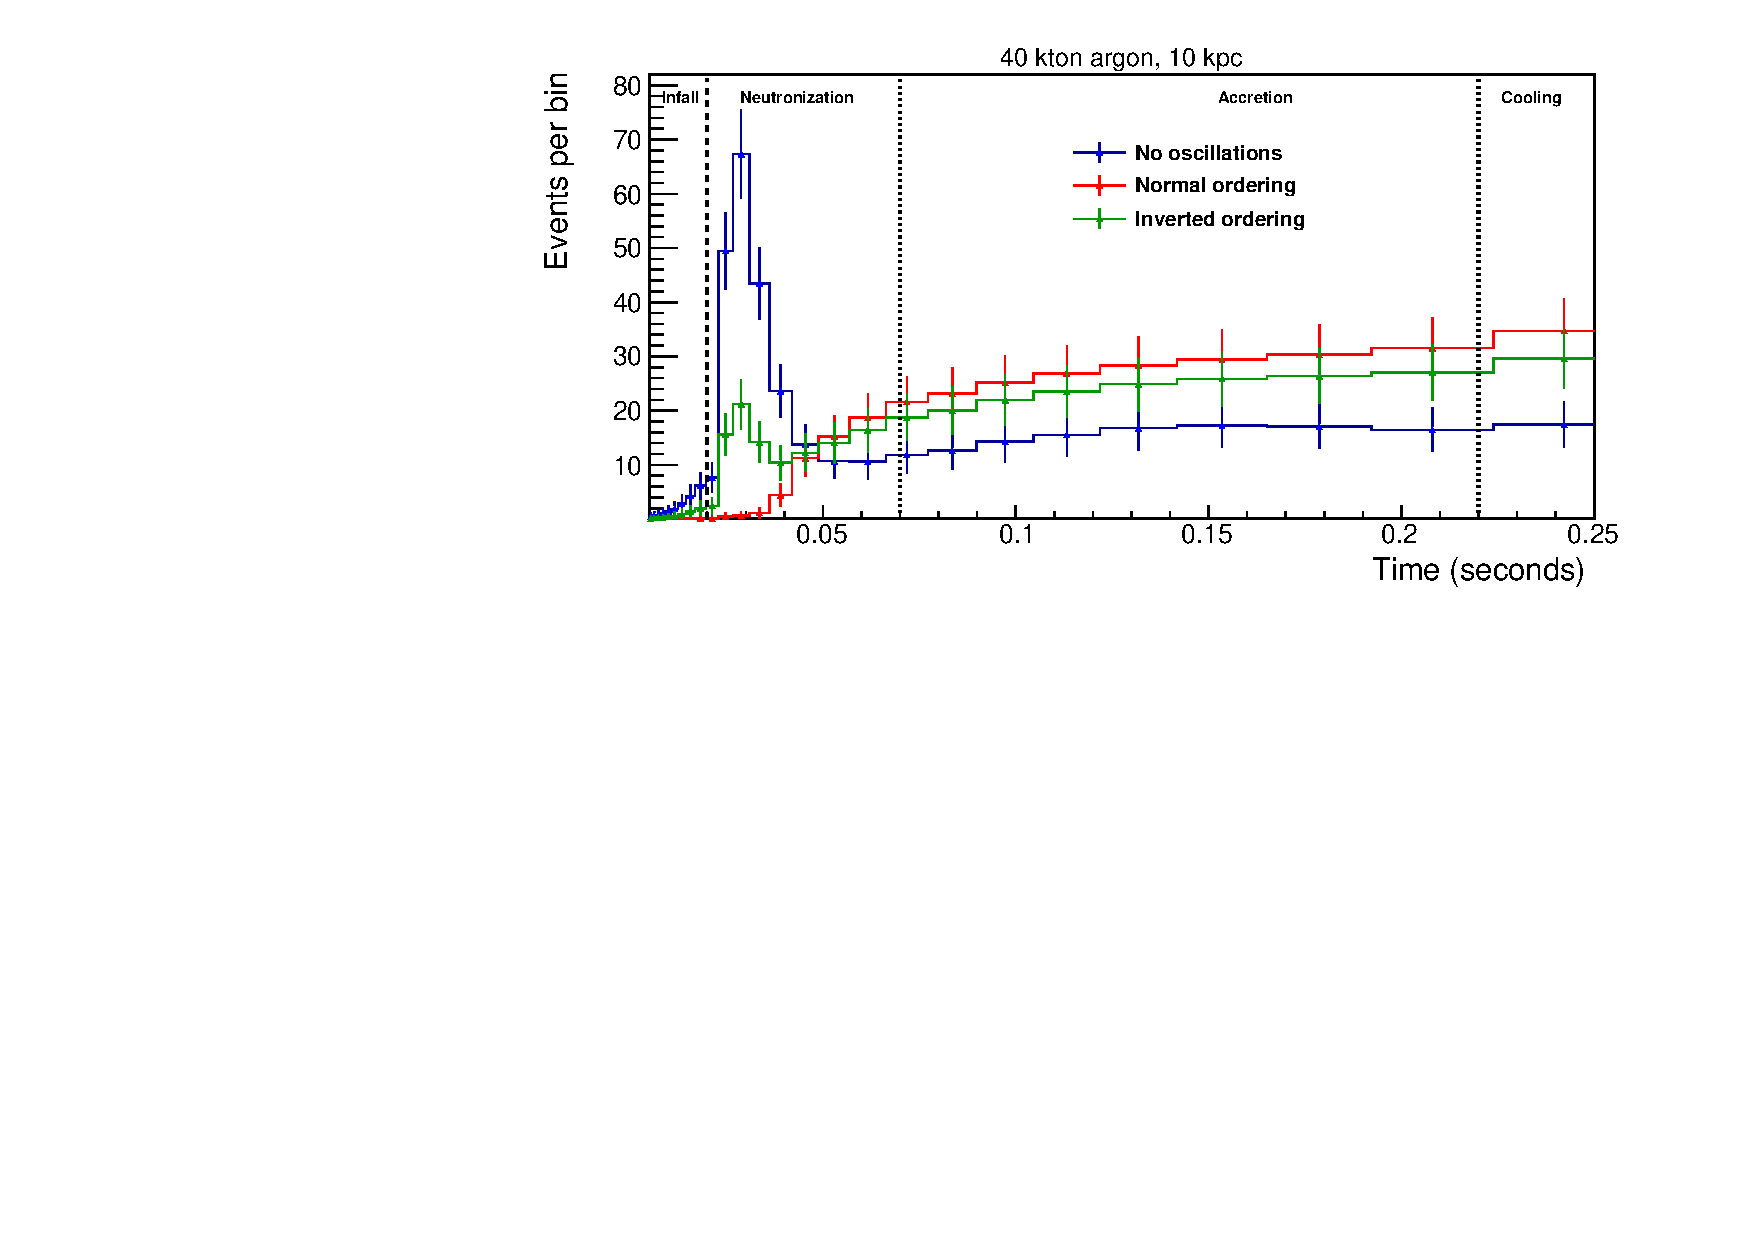
\includegraphics[width=0.8\textwidth]{early_time_argon.pdf}
\end{dunefigure}

Of course, if mass hierarchy is already known, we can turn it around 
and use the terrestrial determination to better disentangle the other 
particle physics and astrophysics knowledge. 


%Matter effects in the Earth can also have a mass-hierarchy-dependent effect on the signal (e.g.,~\cite{Choubey:2010up}).


Figure~\ref{fig:neutronization_mh} shows the results of a simple quantitative study
based in counting observed events in DUNE in the first 50 milliseconds
of the burst.  We expect this early neutronization-burst period to be
dominated by adiabatic \dword{msw} transitions driven by the ``H-resonance''
for $\Delta m^2_{3\ell}$, for which the following
neutrino-energy-independent relations apply:

\begin{eqnarray}  
 F_{\nu_e} &=& F^0_{\nu_x} \,\ \,\ \,\ \,\ \,\ \,\ \,\ \,\  \,\ \,\ \,\ \,\   \,\ \,\  \,\ \,\ \,\ \,\ \,\ \,\  \,\ \,\ \textrm{(\dword{nh})} \,\ , \label{eq:msw_nmo}\\
 F_{\nu_e} &=&  \sin^2 \theta_{12} F^0_{\nu_e} +
\cos^2 \theta_{12} F^0_{\nu_x}  \,\ \,\ \,\ \,\ \textrm{(\dword{ih})} \,\,
\label{eq:msw_imo}
\end{eqnarray} 
 and 
\begin{eqnarray}  
 F_{\bar\nu_e} &=& \cos^2 \theta_{12} F^0_{\bar\nu_e} + \sin^2 \theta_{12} F^0_{\bar\nu_x}   \,\   \,\ \,\  \,\ \,\ \,\ \,\ \,\ \,\  \,\ \,\ \textrm{(\dword{nh})} \,\ , \label{eq:msw_nmo_anti}\\
 F_{\bar\nu_e} &=&   F^0_{\bar\nu_x}  \,\ \,\ \,\ \,\ \,\ \,\ \,\ \,\ \,\ \,\ \,\ \,\ \,\ \,\ \,\ \,\ 
 \,\ \,\ \,\ \,\ \,\ \,\ \,\ \,\ \,\ \,\ \,\ \,\ \,\  \,\
\textrm{(\dword{ih})} \,\,\label{eq:msw_imo_anti}
\end{eqnarray} 

where $F$'s are the fluxes corresponding to the respective flavors,
and the $^o$ subscript represents flux before transition.

% From Vitor
\begin{dunefigure}[MH1]{fig:neutronization_mh}{Event counts in the
    first 50 milliseconds for the model in~\cite{Huedepohl}, under
    assumptions of no oscillations, normal hierarchy and inverted
    hierarchy, assuming adiabatic \dword{msw} transitions.  The left plot
    shows the event number as a function of distance with statistical
    errors.  The right plot
    shows the event number scaled by square of distance, under the
    assumption of a 20\% uncertainty on distance. }
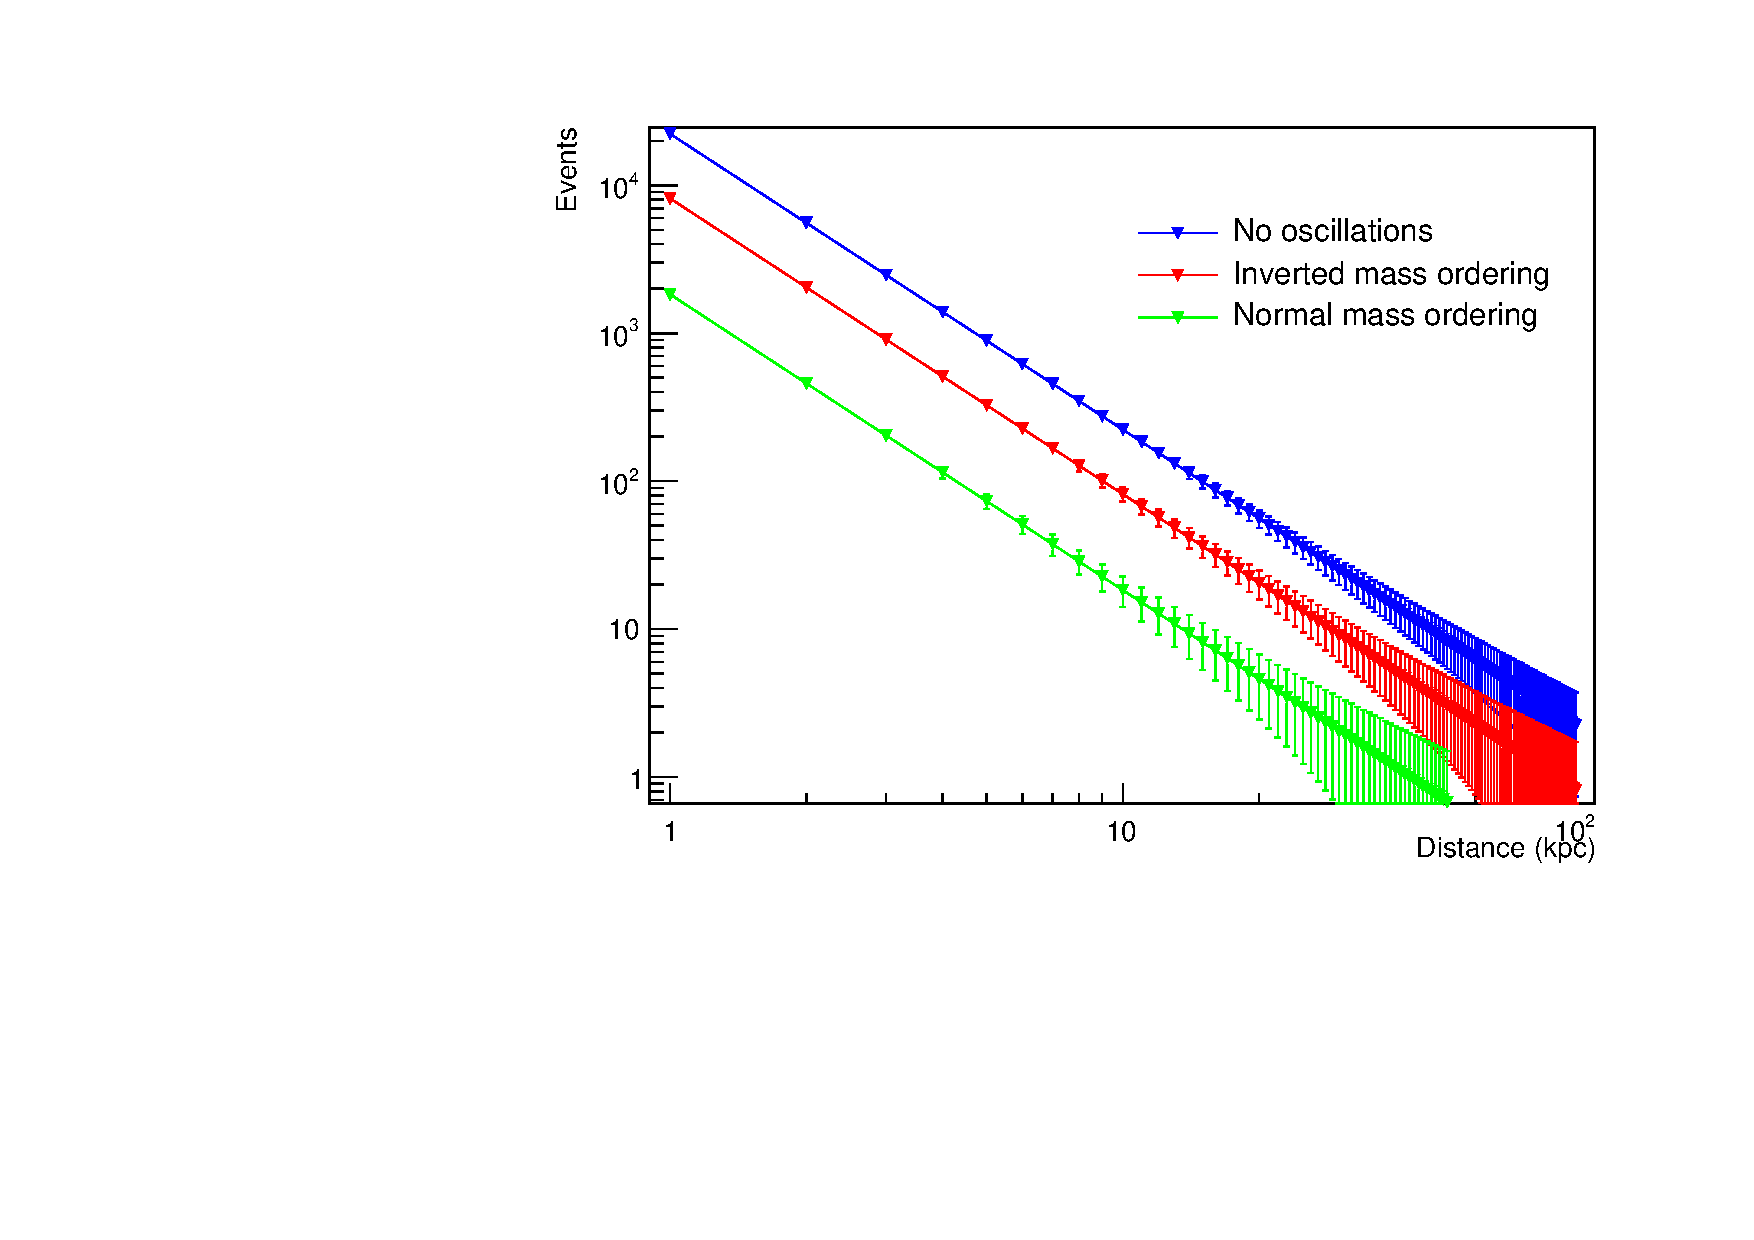
\includegraphics[width=3.2in]{event_distance_logxy.pdf}
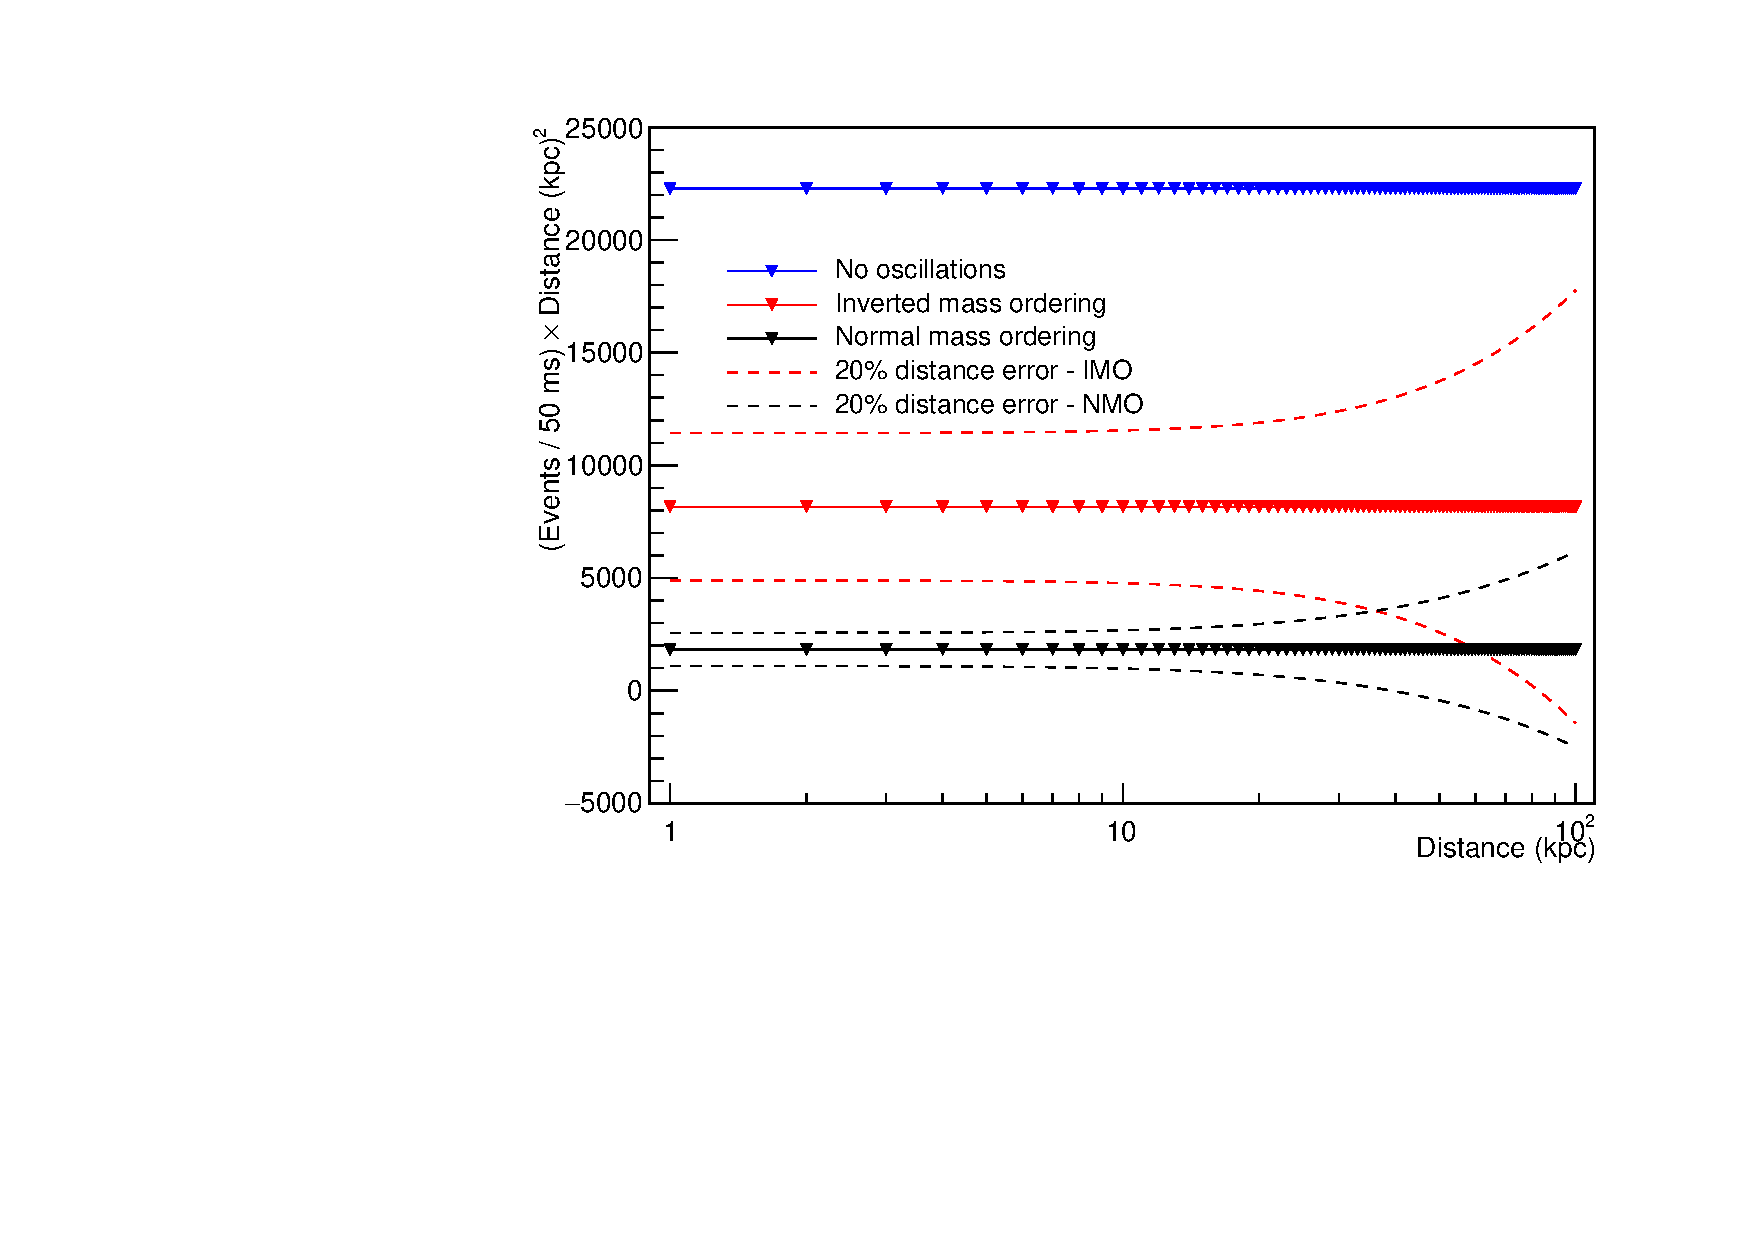
\includegraphics[width=3.2in]{MO_distance_errors_20.pdf}
\end{dunefigure}

Figure~\ref{fig:neutronization_mh} shows that the event count will be
well separated under the two different assumptions, out to the edge of
the Galaxy for this model.  The right hand plot shows also the effect of uncertainty
on the distance to the supernova, in the scenario of evaluating the
mass hierarchy based on absolute neutronization-burst counts (however
note that there will be additional information on expected scale of
the signal from other time eras of the signal). \textit{There may be
  updates to this study incorporating a range of models and using
  different discriminants.}


\subsection{Lorentz Invariance Violation}

% From Alan Kostelecky
As another example of a probe of new physics with supernova neutrinos or antineutrinos,
a class of tests of Lorentz and \dword{cpt} violation involves comparing the propagation of neutrinos with other species of neutrinos of the same flavor but different energies~\cite{Kostelecky:2003cr,Kostelecky:2003xn,Kostelecky:2011gq,Diaz:2009qk}. These amount to time-of-flight or dispersion studies.
Time-of-flight and dispersion effects lack the interferometric resolving power available to neutrino oscillations, but they provide instead sensitivity to Lorentz- and \dword{cpt}-violating effects that  leave unaffected neutrino oscillations
and so cannot be measured using atmospheric or long-baseline neutrinos.
The corresponding \dword{sme} coefficients controlling these effects are called oscillation-free coefficients~\cite{Kostelecky:2011gq}.

Supernova neutrinos are of particular interest in this context because of the long baseline, which implies sensitivities many orders of magnitude better than available from time-of-flight measurements in beams. Observations of the supernova SN1987A yield constraints on the difference between the speed of light and the speed of antineutrinos, which translates into constraints on isotropic and anisotropic coefficients in both the minimal and nonminimal sectors of the \dword{sme}. Knowledge of the spread of arrival times constrains the maximum speed difference between SN1987A antineutrinos of different energies in the approximate range 10--40 MeV, which restricts the possible antineutrino dispersion and yields further constraints on \dword{sme} coefficients~\cite{Kostelecky:2011gq}.

Analyses of this type would be possible with DUNE if supernova neutrinos are observed. Key features to maximize sensitivity would include absolute timing information to compare with photon spectral observations (and perhaps ultimately with gravitational-wave data~\cite{Kostelecky:2016kfm})  along with relative timing information for different components of the neutrino energy spectrum. Significant improvements over existing limits are possible.

Figure \ref{fig:livsn} displays DUNE supernova sensitivities 
to these relevant oscillation-free coefficients 
for Lorentz and \dword{cpt} violation.
The estimated sensitivities are obtained using
the general expression (125) in ~\cite{Kostelecky:2011gq}
for the neutrino velocity in oscillation-free models
and its application (132) to dispersion studies.
The figure assumes a supernova comparable to SN1987A
and at the same location on the sky.
Enhancements of the displayed sensitivities 
from angular factors can occur for different sky locations.
Studies of supernova neutrinos using DUNE 
can measure many coefficients (green) 
at levels improving over existing limits (gray).

\begin{dunefigure}[DUNE SN sensitivities to oscillation-free coefficients for Lorentz and \dword{cpt} violation]{snliv}{DUNE supernova sensitivities to oscillation-free coefficients for Lorentz and \dword{cpt} violation. Studies of DUNE supernova neutrinos can measure many coefficients (green) at levels improving over existing limits (grey). These Lorentz- and \dword{cpt}- violating effects leave oscillations unchanged and so are challenging to detect in atmospheric or long-baseline measurements~\cite{kostelecky}.\label{fig:livsn}}
\includegraphics[width=0.9\textwidth]{liv-sn.pdf}
\end{dunefigure}

Finally, via detection of time-of-flight delayed $\nu_e$ from the  neutronization burst,  DUNE will be able to probe neutrino mass bounds of $\mathcal{O}(1)$~eV for a 10-kpc supernova~\cite{Rossi-Torres:2015rla} (although likely not competitive near-future terrestrial kinematic limits).  If eV-scale sterile neutrinos exist, they will likely have an impact on astrophysical and oscillation aspects of the signal (e.g.,~\cite{Keranen:2007ga,Tamborra:2011is,Esmaili:2014gya}), as well as time-of-flight observables. \\





\section{Additional Astrophysical Neutrinos}
\label{sec:physics-snblowe-other}

\subsection{Solar Neutrinos}

Intriguing questions in solar neutrino physics remain,
even after data
from the \dword{sk} and \dword{sno}~\cite{Fukuda:2001nj,Ahmad:2001an}
experiments explained the long-standing mystery of missing solar
neutrinos~\cite{Cleveland:1998nv} as due to flavor
transformations. 
Some unknowns, such as the fraction of energy production via the \dword{cno}
cycle in the Sun, flux variation due to helio-seismological modes that
reach the solar core, or long-term stability of the solar core
temperature, are astrophysical in nature. Others directly impact
particle physics. Can the \dword{msw} model explain the amount of flavor
transformation as a function of energy, or are non-standard neutrino
interactions required?  Do solar neutrinos and reactor antineutrinos
oscillate with the same parameters?   Interesting observables are the
day/night effect, and potentially the hep flux.

Detection of solar and other low-e.nergy neutrinos is challenging in
a \dword{lartpc} because of relatively high intrinsic detection energy thresholds for
the charged-current interaction on argon ($>$\SI{5}{\MeV}). 
Compared with other technologies, a \dword{lartpc} offers a large
cross section and unique potential signatures from deexcitation
photons. Aggressive R\&D efforts in low-energy triggering and
control of background from radioactive elements may make detection
of solar neutrinos in DUNE possible.

Signatures of solar neutrinos in DUNE
are elastic scattering on electrons as well as \dword{cc} absorption of $\nu_e$ on $^{40}$Ar (equation~\ref{eq:nueabs}), which has a 4.5-MeV energy threshold and a large cross section compared to elastic scattering on electrons.  Furthermore, the \dword{cc} absorption differential cross section (the interaction products track neutrino energy closely) potentially enables precise solar-neutrino spectral measurements.
The solar neutrino event rate in a
\ktadj{40} \dword{lartpc}, assuming a \MeVadj{4.5} neutrino energy
threshold and 31\% $\nu_e$ survival, is 122 per day.

Reference~\cite{Capozzi:2018dat} explores the solar neutrino potential
of DUNE, with somewhat optimistic energy resolution assumptions.

% The solar neutrino physics potential of a large \dword{lartpc} depends
% on the ability to pick up a low-energy electron, light collection of the photon-triggering system,
% and, critically, on background suppression. 
% The decay of the naturally occurring $^{39}$Ar
% produces $\beta$'s with a \keVadj{567} endpoint and an expected rate
% of \SI{10}{\MHz} per \SI{10}{\kt} of liquid argon. This limits the
% fundamental reach of DUNE to neutrino interactions with visible
% energies above \SI{1}{\MeV}. 
% Cosmic-muon and fast-neutrino  interactions with the $^{40}$Ar nucleus (which are rather complex
% compared to interactions on $^{16}$O or $^{12}$C) are likely to generate many long-lived spallation products which could limit the
% detection threshold for low-energy neutrinos.
% $^{40}$Cl, a beta emitter with an
% endpoint of \SI{7.48}{\MeV}, is a dominant source of background at
% energies above \SI{5}{\MeV}, and is expected to be produced with a rate on the order of 10 per kton of LAr per day at 4850 ft.



% The ICARUS collaboration has reported a \MeVadj{10}
% threshold~\cite{Guglielmi:2012}. Assuming the detector itself
% has low enough radioactivity levels, this threshold level would enable
% a large enough detector to measure the electron flavor component of
% the solar $^8$B neutrino flux with high statistical accuracy. It could 
% thereby further test the \dword{msw} flavor transformation curve with higher statistical precision and
% potentially better energy resolution. 
% In addition to these solar
% matter effects, solar 
% neutrinos also probe terrestrial matter effects
% with the variation of the $\nu_e$ flavor observed with solar zenith
% angle while the Sun is below the horizon --- the day/night effect (reported recently in ~\cite{Renshaw:2013dzu}). 
% The comparison
% of neutrino disappearance to antineutrino disappearance tests \dword{cpt}
% invariance. 


\subsection{Diffuse Supernova Background Neutrinos}

Galactic supernovae are relatively rare, occurring somewhere between
once and four times a century. In the Universe
at large, however, thousands of neutrino-producing explosions occur
every hour.  The resulting neutrinos --- in fact most of the neutrinos
emitted by all the supernovae since the onset of stellar formation ---
suffuse the Universe.  Known as the %\emph{diffuse supernova neutrino background
 % (DSNB)}
\dword{dsnb}, their energies are in the few-to-\MeVadj{30} range.  \dword{dsnb}
have not yet been observed, but an observation would greatly enhance
our understanding of supernova-neutrino emission and the overall
core-collapse rate~\cite{Beacom:2010kk}.


A liquid argon detector such as DUNE's far detector is sensitive to
the $\nu_e$ component of the diffuse relic supernova neutrino flux,
whereas water Cherenkov and scintillator detectors are sensitive to
the antineutrino component.  However, backgrounds in liquid argon are as
yet unknown, and a huge exposure ($>$\SI{500}{\ktyr}s)
would likely be required for observation.  
With tight control of
backgrounds, 
DUNE --- in the long term --- could 
lay a unique and
 complementary role in the physics of relic neutrinos.


Background is a serious issue for \dword{dsnb} detection.
The solar {\em hep} neutrinos, which have an                
endpoint at \SI{18.8}{\MeV}, will determine the lower bound of the \dword{dsnb}
search window ($\sim$ \SI{16}{\MeV}).  The upper bound is determined
by the atmospheric ${\nu}_{e}$ flux and
is around \SI{40}{MeV}.
Although the \dword{lartpc} provides a unique sensitivity to the
electron-neutrino component of the \dword{dsnb} flux, early studies indicate
that due to this lower bound of $\sim$ \SI{16}{\MeV} DUNE would need a huge
mass of liquid argon --- of order \SI{100}{\kt} --- to get more than 4$\sigma$
evidence for the diffuse supernova flux in five
years~\cite{Cocco:2004ac}.
%
The expected number of relic
supernova neutrinos, $N_{\rm \dword{dsnb}}$, that could be observed in a
\SIadj{40}{\kt} \dword{lartpc} detector in ten years~\cite{Cocco:2004ac}
assuming normal hierarchy is:
\begin{equation}
N_{\rm \dword{dsnb}} = 46 \pm 10  \ \ \ 16 \, {\rm MeV} \leq E_e \leq 40 \, {\rm MeV}
\label{eqn:srnrate}
\end{equation}
where $E_e$ is the energy of the electron from the \dword{cc}. interaction as
shown in Equation~\ref{eq:nueabs}. 

 The main challenge for detection of such
a low rate of relic neutrinos in a \dword{lartpc} is understanding how much of
the large spallation background from cosmic-ray interactions with the
heavy argon nucleus 
leaks into the search window.   Some studies have been done~\cite{Barker:2012nb} but more work is needed.

\subsection{Other Low-Energy Neutrino Sources}

We note some other potential sources of signals in the tens-of-MeV
range which may be observable in DUNE.  A small flux is expected from
Type I (thermonuclear) supernovae~\cite{Wright:2016gar,
  Wright:2016xma}, with potential detectability by DUNE within a few
kpc.   Other signals include neutrinos from accretion disks~\cite{Caballero:2011dw} and black-hole/neutron star mergers~\cite{Caballero:2009ww}.  These will create spectra not unlike those from core-collapse events, and with potentially large fluxes.  However they are expected to be considerably rarer than core-collapse supernovae within an observable distance range.  There may also be signatures of dark-matter \dword{wimp}. annihilations in the low-energy signal range~\cite{Rott:2012qb, Bernal:2012qh}.



\section{Detector Requirements}
\label{sec:physics-snblowe-detector-requirements}

For supernova burst physics, the detector must be able to detect and reconstruct as well as possible events in the range 5--100~MeV.  As for proton decay and atmospheric neutrinos, no beam trigger will be available; therefore there must be special triggering and \dword{daq} requirements that take into account the short, intense nature of the burst, and the need for prompt propagation of information in a worldwide context.
The DUNE Far Detector
Requirements~\cite{lbnfdune-cdr-req} specific to supernova burst neutrinos are as follows:

\begin{itemize}

  % This seems obsolete; depth is fixed.
% \item Far Detector Depth: The signal to background ratio shall be sufficiently large to identify the  burst ($<$100 seconds)  from a core-collapse supernova within 20~kpc (within the Milky Way). This will require a detector located at sufficient depth for cosmic-ray-related background, including spallation-induced events, to be sufficiently low.  Furthermore backgrounds from radioactivity or other sources must also be sufficiently low.  Preliminary studies~\cite{gehman} indicate that backgrounds at 4850 ft (including both cosmogenics and intrinsic radioactivity) will be sufficiently low, although more work is needed.

\item Far Detector Triggering and \dword{daq}:  The far detector shall
  be capable of collecting information for a supernova burst within
  the Milky Way.  Events are expected within a time window of
  approximately 30 seconds, but possibly over an interval as long as a
  few hundred seconds; a large fraction of the events are expected within approximately the first second of the burst.
The data acquisition buffers shall be sufficiently large and the data acquisition system sufficiently robust to allow full capture of neutrino event information for a supernova as close as 0.1 kpc.
At 10~kpc, one expects thousands of events within approximately 10 seconds, but a supernova at a distance of less than 1~kpc would result in $10^5-10^7$  events over 10 seconds.    

The far detector shall have high uptime ($>$99.5\%) with little event-by-event deadtime to allow the capture of low-probability astrophysical events that could occur at any time with no external trigger. 
Supernova events are expected to occur a few times per century within the Milky Way galaxy. For any 10-year period, the probability of a supernova could be 20 to 30\%.  Capturing such an event at the same time as many of the other detectors around the Earth is very important.  

The DUNE detector systems shall be configured to provide information
to other observatories on possible astrophysical events (such as a
galactic supernova) in a short enough time to allow global
coordination.  This interval should be less than 30 minutes, and
preferably
on a few-minute timescale.  To obtain maximum scientific value out of a singular
astronomical event, it is very important to inform all other
observatories (including optical ones) immediately via SNEWS~\cite{snews}, so that they can
begin observation of the evolution of the event. Pointing information
should also be made available as promptly as possible.

\item Far Detector Event Reconstruction:   
The far detector shall be capable of collecting low energy ($<$\SI{100}{\MeV})  charged-current electron neutrino interactions on $^{40}$Ar nuclei that arrive in a short period of time. The final-state electron (or positron) shall be detected and its energy measured.   An energy threshold of 5 MeV or better is highly desirable; most supernova burst events are expected to have energy depositions in the range 5--50~MeV.
Energy and event time resolution must be sufficient to resolve
interesting physics features of the burst.  Knowledge of detector
parameters such as energy resolution, energy scale, and energy threshold
as well as understanding of cross sections, are important to avoid biases
in supernova flux parameter determination.
Time resolution of $\mu$s should be sufficient to resolve burst time features.


%Preliminary studies
%suggest that resolution measured by Icarus for low-energy
%events~\cite{Amoruso:2003sw} should be adequate, and that
%approximately 10~$\mu$s event time resolution should be sufficient to resolve features such as the neutronization burst and the preceding short notch due to neutrino trapping in the $\nu_e$ spectrum (see the luminosity curve of Figure~\ref{fig:garching}), given adequate statistics.   
%Detection of gamma ray photons from the final-state excited nucleus could lead to additional electronics requirements.  

\end{itemize}



The other low-energy physics described in Sections~\ref{sec:physics-snblowe-other} typically requires similar event reconstruction capabilities as does supernova-burst physics; however background requirements are much more stringent for these (especially for \dword{dsnb}).  Realistic background conditions in the few-tens-of-MeV range are not currently  very well understood.  
These physics topics do not drive detector requirements, although it may still be possible for DUNE to address them if backgrounds can be kept sufficiently well under control.




%\subsection{Triggering and \dword{daq}}

%This will be a summary of the relevant part of the TDR.


